% Necoyoad Architecture Blueprint v3 — Theme & Widget Rendering Pipeline
% Deep dive into the presentation layer, verified against the PHP source.

\documentclass[11pt,a4paper]{article}

% ============================================================
%  Packages
% ============================================================
\usepackage[T1]{fontenc}
\usepackage[utf8]{inputenc}
\usepackage{lmodern}
\usepackage{microtype}

\usepackage{graphicx}
\usepackage{xcolor}
\usepackage{geometry}
\usepackage{amsmath}
\usepackage{amssymb}

\usepackage{tcolorbox}
\tcbuselibrary{skins,breakable,listings}
\usepackage{colortbl}
\usepackage{booktabs}
\usepackage{tabularx}
\usepackage{longtable}
\usepackage{array}
\usepackage{enumitem}
\usepackage{adjustbox}
\usepackage{caption}
\usepackage{fancyhdr}
\usepackage{titlesec}
\usepackage{pdflscape}
\usepackage{listings}

% TikZ
\usepackage{tikz}
\usetikzlibrary{arrows.meta,positioning,calc,shapes.geometric,fit,backgrounds,chains,decorations.pathreplacing,shapes.multipart}

% hyperref - last
\usepackage[
    colorlinks=true,
    linkcolor=blue!50!black,
    citecolor=blue!40!black,
    urlcolor=blue!60!black,
    bookmarks=true,
    bookmarksnumbered=true,
    unicode=true,
    pdftitle={Necoyoad - Theme & Widget Rendering Pipeline (v3)},
    pdfauthor={Reverse-Engineered Architecture Report},
    pdfsubject={Software Architecture, Presentation Layer, Theme System, Widget Rendering, PHP Source Analysis},
    pdfkeywords={Necoyoad, OpenCart, PHP 8.1, Front Controller, Composite View, Widget Pipeline, NecoWidget, Theme System, EAV Property, deps.php, Hooks, Events, Visual Editor}
]{hyperref}

% ============================================================
%  Page geometry
% ============================================================
\geometry{a4paper, top=2.4cm, bottom=2.4cm, left=2.4cm, right=2.4cm}
\setlength{\headheight}{14pt}

% ============================================================
%  Headings / header-footer
% ============================================================
\pagestyle{fancy}
\fancyhf{}
\fancyhead[L]{\small\itshape Necoyoad v3 --- Theme \& Widget Rendering Pipeline}
\fancyfoot[C]{\small\thepage}
\renewcommand{\headrulewidth}{0.3pt}
\renewcommand{\footrulewidth}{0pt}

\titleformat{\section}{\Large\bfseries\color{black!85}}{\thesection}{0.6em}{}
\titleformat{\subsection}{\large\bfseries\color{black!80}}{\thesubsection}{0.6em}{}
\titleformat{\subsubsection}{\normalsize\bfseries\color{black!75}}{\thesubsubsection}{0.5em}{}

\widowpenalty=10000
\clubpenalty=10000
\emergencystretch=4em
\hbadness=10000
\hfuzz=2pt
\vfuzz=2pt
\sloppy

% ============================================================
%  Colors
% ============================================================
\definecolor{necoyoad-blue}{HTML}{1F4E79}
\definecolor{necoyoad-orange}{HTML}{B85C00}
\definecolor{necoyoad-green}{HTML}{2E6B33}
\definecolor{necoyoad-purple}{HTML}{5B2A86}
\definecolor{nodefill}{HTML}{F4F7FB}
\definecolor{nodefillalt}{HTML}{FBF4EE}
\definecolor{nodefillgreen}{HTML}{F2F8F2}
\definecolor{nodefillpurple}{HTML}{F5EFFA}
\definecolor{nodefillgray}{HTML}{F0F0F2}
\definecolor{phpline}{HTML}{F8F8F0}
\definecolor{phpcomment}{HTML}{8C8C8C}
\definecolor{phpkeyword}{HTML}{1F4E79}
\definecolor{phpstring}{HTML}{B85C00}

% ============================================================
%  PHP code listing style
% ============================================================
\lstdefinelanguage{necophp}{
  morekeywords={abstract,and,array,as,break,case,catch,class,clone,const,continue,declare,default,do,echo,else,elseif,empty,enddeclare,endfor,endforeach,endif,endswitch,endwhile,extends,final,finally,for,foreach,function,global,goto,if,implements,include,include_once,instanceof,insteadof,interface,namespace,new,or,print,private,protected,public,require,require_once,return,static,switch,throw,trait,try,use,var,while,xor,yield,true,false,null},
  sensitive=true,
  morecomment=[l]{//},
  morecomment=[s]{/*}{*/},
  morecomment=[l]{\#},
  morestring=[b]",
  morestring=[b]',
}
\lstset{
  language=necophp,
  basicstyle=\ttfamily\footnotesize,
  keywordstyle=\color{phpkeyword}\bfseries,
  commentstyle=\color{phpcomment}\itshape,
  stringstyle=\color{phpstring},
  backgroundcolor=\color{phpline},
  numbers=left,
  numberstyle=\tiny\color{phpcomment},
  numbersep=8pt,
  frame=single,
  rulecolor=\color{black!25},
  framerule=0.3pt,
  breaklines=true,
  breakatwhitespace=true,
  showstringspaces=false,
  captionpos=b,
  xleftmargin=14pt,
  xrightmargin=4pt,
  aboveskip=8pt,
  belowskip=8pt,
}

% ============================================================
%  tcolorbox styles
% ============================================================
\newtcolorbox{infobox}[1][]{
  enhanced, breakable,
  colback=nodefill, colframe=necoyoad-blue!60,
  boxrule=0.4pt, arc=2pt, left=8pt, right=8pt, top=6pt, bottom=6pt,
  fonttitle=\bfseries\small, coltitle=white,
  title=#1
}
\newtcolorbox{correctionbox}[1][]{
  enhanced, breakable,
  colback=nodefillalt, colframe=necoyoad-orange!70,
  boxrule=0.4pt, arc=2pt, left=8pt, right=8pt, top=6pt, bottom=6pt,
  fonttitle=\bfseries\small, coltitle=white,
  title=#1
}

\captionsetup{justification=raggedright, singlelinecheck=false, font=small, labelfont=bf}

% ============================================================
\begin{document}

\thispagestyle{empty}

\begin{center}
{\Large\bfseries Necoyoad --- Theme \& Widget Rendering Pipeline (v3)}\\[0.4em]
{\small\itshape A focused deep-dive into the presentation layer:\\
how a controller return becomes HTML, verified against the PHP source}\\[1.2em]
\end{center}

\begin{abstract}
\noindent
This is the third volume of the Necoyoad architecture blueprint. v1
reconstructed the platform from the SQL dump alone. v2 verified v1
against the full PHP source. v3 zooms in on a single subsystem ---
the \emph{presentation layer} --- and traces, in exhaustive detail,
how a controller's return value becomes the final HTML that reaches
the browser.

The presentation layer is the most intricate part of Necoyoad. It
combines: (i) a composite-view pattern where every page is assembled
from a parent template plus layout children (header, footer,
columns) plus widget children; (ii) a string-based
\texttt{\{\%widget\_name\%\}} placeholder substitution mechanism
that runs \emph{after} template rendering; (iii) a
database-backed widget system where widget instances, rows, and
columns are stored in the polymorphic \texttt{property} EAV table
and queried with \texttt{LIKE '\%key=value\%'} predicates against
the serialised settings blob; (iv) a route-aware asset loader
that maps \texttt{?r=store/product} to \texttt{storeproduct.css}
and \texttt{storeproduct.js} by string convention; (v) a
\texttt{deps.php} manifest that declares which CSS/JS files apply
to which routes; (vi) a dual Hooks/Events extension system with
short-circuit seams at \texttt{render}, \texttt{fetch},
\texttt{loadWidgets}, and \texttt{loadAssets}; (vii) a
device-detection layer that swaps the active theme for mobile,
tablet, or Facebook in-app browsers; (viii) a visual theme editor
that annotates every widget wrapper with \texttt{nt-editable},
\texttt{data-widget}, \texttt{data-position} attributes; and
(ix) a \texttt{theme\_style} CSS-rule override table that lets
the admin write CSS at the selector/property/value granularity
without editing any files.

This paper documents all nine aspects, with 16 verbatim PHP code
listings, 8 TikZ diagrams, a full rendering-pipeline trace (33
steps from \texttt{web/index.php} entry to \texttt{Response::output()}
final emission), and the complete 69-module listing. The stance
is unchanged from v1 and v2: \textbf{descriptive, not prescriptive}.
No improvements are proposed.
\end{abstract}

\vspace{0.6em}
\noindent\textbf{Keywords:} Necoyoad, OpenCart lineage, PHP 8.1.2,
Composite View pattern, widget pipeline, NecoWidget, EAV property
table, \texttt{LIKE '\%key=value\%'} queries, route-aware asset
loader, \texttt{deps.php} manifest, Hooks/Events dual system,
device detection, visual theme editor, \texttt{theme\_style} CSS
overrides, choroni theme.

\newpage
\tableofcontents
\newpage

% ============================================================
\section{Introduction and Scope}\label{sec:intro}
% ============================================================

\subsection{Three Volumes, Three Scales}

This is the third volume of the Necoyoad architecture blueprint.
The three volumes operate at different scales:

\begin{itemize}[leftmargin=1.6em,itemsep=2pt]
  \item \textbf{v1 --- SQL-only reconstruction.} 35 pages. The whole
        platform reverse-engineered from the 87-table database dump.
        Every inference labelled as such.
  \item \textbf{v2 --- Source verification.} 35 pages. v1's inferences
        verified against the 1,450-file PHP source. 8 confirmed,
        2 corrected, 1 partial. Adds the bootstrap, the engine, the
        dual Hooks/Events system, the actual password algorithm, the
        order source code, the cron CLI, the admin REST API.
  \item \textbf{v3 --- This volume.} A single-subsystem deep dive.
        The presentation layer only. How a controller's return value
        becomes the HTML the browser receives.
\end{itemize}

\subsection{Why the Presentation Layer?}

The presentation layer is the most intricate part of Necoyoad. It is
where seven distinct mechanisms interlock:

\begin{enumerate}[leftmargin=1.6em,itemsep=2pt]
  \item \textbf{Composite view.} Every page is a parent template
        plus layout children (header, footer, columns) plus widget
        children. The composition is recursive: a layout child
        itself calls \texttt{render()}, which itself iterates
        children.
  \item \textbf{String-based placeholder substitution.} Widget
        output is inserted into the parent template by
        \texttt{str\_replace('\{\%widget\_name\%\}', \$output,
        \$content)} \emph{after} the template has been required.
        This is a post-render substitution, not a tree-based
        composition.
  \item \textbf{Database-backed widget tree.} Widget instances,
        rows, and columns are stored in the polymorphic
        \texttt{property} EAV table. Queries use
        \texttt{LIKE '\%key=value\%'} predicates against the
        serialised settings blob.
  \item \textbf{Route-aware asset loader.} The route
        \texttt{?r=store/product} is mapped by string convention
        to \texttt{storeproduct.css} and \texttt{storeproduct.js}.
        A \texttt{deps.php} manifest declares which routes get
        which assets.
  \item \textbf{Dual Hooks/Events extension system.} Hooks
        (WordPress-style, short-circuit on truthy return) fire at
        \texttt{render}, \texttt{fetch}, \texttt{loadWidgets},
        \texttt{loadAssets}, \texttt{redirect}, \texttt{index},
        \texttt{async}, \texttt{csspath}, \texttt{jspath},
        \texttt{loadcss}, \texttt{loadstyles}, \texttt{loadjavascripts},
        \texttt{processcss}, \texttt{rowcss}, \texttt{columncss},
        \texttt{widget:settings}, \texttt{module:settings}. Events
        (Node-style, no short-circuit) fire at \texttt{beforeLoad},
        \texttt{afterLoad}, \texttt{beforeRender}, \texttt{afterRender},
        \texttt{beforeLoadWidget}, \texttt{loadWidget},
        \texttt{renderWidget}, \texttt{addChild}, \texttt{dispatch}.
  \item \textbf{Device detection and theme swapping.} The
        \texttt{Browser} library classifies the request as mobile,
        tablet, Facebook in-app, or desktop. Each class can either
        redirect to a separate URL or swap \texttt{config\_template}
        to a per-device theme.
  \item \textbf{Visual theme editor.} Every widget wrapper carries
        \texttt{nt-editable="1"}, \texttt{data-widget},
        \texttt{data-position}, \texttt{data-necotienda\_module}
        attributes. The editor's JS scans the DOM for these and
        attaches click/drag handlers. The \texttt{theme\_style}
        table stores CSS-rule overrides at the
        selector/property/value granularity.
\end{enumerate}

\subsection{Methodology}

Every claim in this paper is verified against the PHP source commit
\texttt{ce75adf} (``first load''). The relevant files are:

\begin{itemize}[leftmargin=1.6em,itemsep=2pt]
  \item \texttt{system/engine/controller.php} (821 lines) ---
        \texttt{render()}, \texttt{fetch()}, \texttt{loadWidgets()},
        \texttt{loadAssets()}, \texttt{addChild()}, \texttt{setvar()},
        \texttt{redirect()}, \texttt{forward()}, and the protected
        state.
  \item \texttt{system/library/template.php} (24 lines) --- the
        legacy \texttt{Template} class.
  \item \texttt{system/library/document.php} (113 lines) --- the
        page-metadata accumulator.
  \item \texttt{system/library/url.php} --- the SEO URL builder.
  \item \texttt{system/library/response.php} --- the final HTML
        emitter (with gzip).
  \item \texttt{system/helper/widgets.php} (785 lines) --- the
        \texttt{NecoWidget} class, the widget data-access object.
  \item \texttt{system/classes/module.php} (107 lines) --- the
        \texttt{Module} base class for storefront widget
        controllers.
  \item \texttt{app/shop/map.php} (329 lines) --- the storefront
        bootstrap (mobile switching, deps.php loading).
  \item \texttt{app/shop/controller/common/home.php} (87 lines),
        \texttt{header.php} (378 lines), \texttt{footer.php},
        \texttt{column\_left.php}, \texttt{column\_right.php},
        \texttt{maintenance.php}.
  \item \texttt{app/shop/controller/module/modulecontroller.php}
        --- the storefront widget base.
  \item \texttt{app/shop/controller/module/banner.php} --- a
        representative storefront widget.
  \item \texttt{app/admin/controller/extension/module.php} ---
        the admin module installer.
  \item \texttt{app/admin/controller/module/widgetcontroller.php}
        --- the admin widget config base.
  \item \texttt{app/admin/controller/style/widget.php} --- the
        widget layout manager.
  \item \texttt{app/admin/controller/style/theme.php} and
        \texttt{app/admin/model/style/theme.php} --- the theme +
        \texttt{theme\_style} CSS generator.
  \item \texttt{app/admin/model/style/widget.php} --- the widget
        DAO.
  \item \texttt{app/shop/view/theme/choroni/} --- the only shipped
        theme (14 top-level folders, 87 \texttt{.tpl} files in
        \texttt{common/}, \texttt{shared/}, \texttt{module/},
        \texttt{store/}, \texttt{account/}, \texttt{checkout/},
        \texttt{content/}, \texttt{payment/}, \texttt{page/},
        \texttt{error/}, \texttt{localisation/}, \texttt{banner/}).
  \item \texttt{web/assets/theme/choroni/css/deps.php} (177 lines)
        and \texttt{web/assets/theme/choroni/js/deps.php}
        (154 lines) --- the asset manifests.
  \item 5 representative admin modules in depth:
        \texttt{banner}, \texttt{category\_list},
        \texttt{product\_overview}, \texttt{shopping\_cart\_box},
        \texttt{google\_analytics}. All 69 module folder names listed
        in Appendix~\ref{app:modules}.
\end{itemize}

\subsection{Document Roadmap}

Section~\ref{sec:overview} gives a 30-second overview.
Section~\ref{sec:engine} covers the rendering engine
(\texttt{Controller::render()} and \texttt{Controller::fetch()}).
Section~\ref{sec:composite-view} explains the composite-view
pattern and the numeric-vs-string child key distinction.
Section~\ref{sec:widget-dao} covers \texttt{NecoWidget} and the
\texttt{LIKE '\%key=value\%'} query pattern.
Section~\ref{sec:assets} covers the route-aware asset loader and
the \texttt{deps.php} manifest.
Section~\ref{sec:layout-composers} walks through the six common
controllers.
Section~\ref{sec:theme} covers the \texttt{choroni} theme, its
folder structure, the shared fragments, and the \texttt{\$tpl}
inheritance mechanism.
Section~\ref{sec:device} covers device detection and theme
switching.
Section~\ref{sec:visual-editor} covers the visual theme editor
hooks and the \texttt{theme\_style} CSS generator.
Section~\ref{sec:hooks-seams} catalogues the 18 hook and 10 event
emit points in the rendering pipeline.
Section~\ref{sec:trace} is the heart: a 33-step rendering-pipeline
trace, from \texttt{web/index.php} entry to
\texttt{Response::output()} final emission, naming every method
call and every table query.
Section~\ref{sec:modules} covers the 69 admin modules.
Section~\ref{sec:observations} closes with non-recommendatory
observations. Appendix~\ref{app:modules} lists all 69 module
folders; Appendix~\ref{app:theme-tree} gives the full theme
folder tree.

% ============================================================
\section{Thirty-Second Overview}\label{sec:overview}
% ============================================================

A request hits \texttt{web/index.php}. The bootstrap loads the
engine, the libraries, the active theme's \texttt{deps.php}
manifest, and the settings. The Front Controller dispatches to
the target route (e.g.\ \texttt{common/home}). The target
controller calls \texttt{loadWidgets()} for each layout position
(\texttt{featuredContent}, \texttt{main}, \texttt{featuredFooter},
\texttt{header}, \texttt{footer}, \texttt{column\_left},
\texttt{column\_right}). \texttt{NecoWidget} queries the
\texttt{property} EAV table for widget rows, columns, and
instances --- using \texttt{LIKE '\%key=value\%'} predicates
against the serialised settings blob. The widgets' routes
(e.g.\ \texttt{module/banner}) are merged into
\texttt{\$this->children} with string keys. The layout children
(\texttt{common/header}, \texttt{common/footer},
\texttt{common/column\_left}, \texttt{common/column\_right}) are
pushed via \texttt{addChild()} with numeric keys.

The controller calls \texttt{render(true)}. \texttt{render()}
runs the \texttt{render} hook (short-circuit), looks up the
cache (keyed by route + device + customer-logged), loads the
route's CSS/JS assets, then iterates the children in FIFO order.
Each child controller's \texttt{index()} runs (which itself calls
\texttt{render()}, recursively). The output is captured and
published into the parent's view-model: numeric-keyed children
become \texttt{\$header}, \texttt{\$footer}, \texttt{\$column\_left},
\texttt{\$column\_right}; string-keyed children become
\texttt{\$<name>\_code} (with a companion \texttt{\$<name>\_hook}
marker).

After the child loop, the parent's own template is fetched:
\texttt{fetch()} injects five magic services into the view-model,
extracts it into local scope, requires the \texttt{.tpl} file, then
runs two passes of \texttt{str\_replace} to substitute
\texttt{\{\%widget\_name\%\}} tokens with the corresponding
\texttt{\$<name>\_code} output. The HTML is post-processed (strip
CSS comments, collapse whitespace, optionally minify), the
\texttt{render} filter is applied, and the result is written to
the cache and to \texttt{Response::output()}.

\begin{figure}[htbp]
\centering
\resizebox{\columnwidth}{!}{%
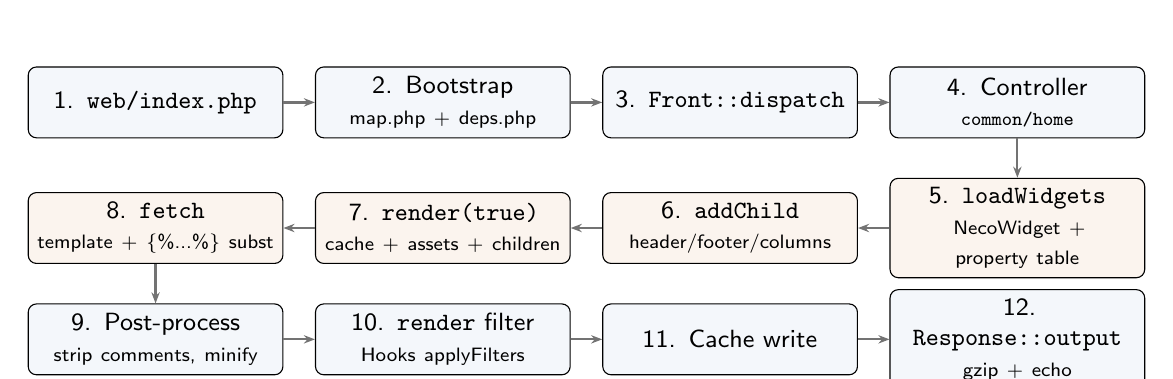
\begin{tikzpicture}[
  box/.style={draw, rounded corners=3pt, text width=3.0cm, minimum height=0.9cm, align=center, font=\small\sffamily, fill=nodefill},
  hotbox/.style={draw, rounded corners=3pt, text width=3.0cm, minimum height=0.9cm, align=center, font=\small\sffamily, fill=nodefillalt},
  arr/.style={-{Stealth[length=4pt]}, thick, black!55}
]
  \node[box] (entry) {1. \texttt{web/index.php}};
  \node[box, right=0.4cm of entry] (boot) {2. Bootstrap\\\scriptsize map.php + deps.php};
  \node[box, right=0.4cm of boot] (dispatch) {3. \texttt{Front::dispatch}};
  \node[box, right=0.4cm of dispatch] (ctrl) {4. Controller\\\scriptsize \texttt{common/home}};

  \node[hotbox, below=0.5cm of ctrl] (loadw) {5. \texttt{loadWidgets}\\\scriptsize NecoWidget + property table};
  \node[hotbox, left=0.4cm of loadw] (addc) {6. \texttt{addChild}\\\scriptsize header/footer/columns};
  \node[hotbox, left=0.4cm of addc] (render) {7. \texttt{render(true)}\\\scriptsize cache + assets + children};
  \node[hotbox, left=0.4cm of render] (fetch) {8. \texttt{fetch}\\\scriptsize template + \{\%...\%\} subst};

  \node[box, below=0.5cm of fetch] (post) {9. Post-process\\\scriptsize strip comments, minify};
  \node[box, right=0.4cm of post] (filter) {10. \texttt{render} filter\\\scriptsize Hooks applyFilters};
  \node[box, right=0.4cm of filter] (cache) {11. Cache write};
  \node[box, right=0.4cm of cache] (output) {12. \texttt{Response::output}\\\scriptsize gzip + echo};

  \draw[arr] (entry) -- (boot);
  \draw[arr] (boot) -- (dispatch);
  \draw[arr] (dispatch) -- (ctrl);
  \draw[arr] (ctrl) -- (loadw);
  \draw[arr] (loadw) -- (addc);
  \draw[arr] (addc) -- (render);
  \draw[arr] (render) -- (fetch);
  \draw[arr] (fetch) -- (post);
  \draw[arr] (post) -- (filter);
  \draw[arr] (filter) -- (cache);
  \draw[arr] (cache) -- (output);
\end{tikzpicture}%
}
\caption{The 12-step rendering pipeline at a glance. Steps 5--8
(the hot boxes) are the heart of the presentation layer: widget
loading, child composition, recursive render, and template fetch
with placeholder substitution. The full 33-step trace is in
Section~\ref{sec:trace}.}
\label{fig:overview}
\end{figure}

% ============================================================
\section{The Rendering Engine}\label{sec:engine}
% ============================================================

The rendering engine lives in \texttt{system/engine/controller.php}.
Two methods do almost all the work: \texttt{render()} and
\texttt{fetch()}. They are recursive: \texttt{render()} calls
each child's \texttt{index()}, which itself calls
\texttt{render()}, which itself calls \texttt{fetch()}.

\subsection{\texttt{Controller::render(\$return = false)}}

The complete order of operations:

\begin{lstlisting}[caption={\texttt{Controller::render()} --- the 8-step algorithm (abridged).},label={lst:render}]
protected function render($return = false) {
    // 1. render action hook (short-circuit)
    $hasToReturn = $this->runHook("render", $this, $return);
    if ($hasToReturn) return $hasToReturn;

    // 2. Resolve cache dependencies
    $cache = $this->registry->get('cache');
    $user  = $this->registry->get('user');
    $browser = $this->registry->get('browser');
    $customer = $this->registry->get('customer');
    $device = '.pc';
    if ($browser->isMobile())    $device = '.mobile';
    elseif ($browser->isTablet())     $device = '.tablet';
    elseif ($browser->isFacebook())   $device = '.facebook';
    if ($this->cacheId) $this->cacheId .= $device . (int)$customer->isLogged();

    // 3. Cache lookup (skipped if admin is logged in)
    if ($this->cacheId && !$user->isLogged()) {
        $cached = $cache->get($this->cacheId, $subKey);
        if ($cached) {
            if ($return) return $cached;
            $this->output = $cached; return;
        }
    }

    // 4. On cache miss --- load own assets (route-specific CSS/JS)
    $this->loadAssets($this->ClassName);
    $this->loadAssets($this->Route);

    // 5. Iterate children in FIFO order
    foreach ($this->children as $key => $child) {
        $action = new Action($child);
        // ... require_once, instantiate, call $controller->index($params)
        // ... capture $output = $controller->output
        if (is_int($key)) {
            // Numeric key: layout child (header, footer, columns)
            $this->data[$controller->id] = $output;  // $header, $footer, ...
        } else {
            // String key: widget child
            $this->data[$key . '_hook'] = $key;
            $this->data[$key . '_code'] = $output;   // {%widget_name%} substitution
        }
    }

    // 6. Render the parent's own template
    $this->trigger('beforeRender', $this->template);
    $r = $this->fetch($this->template);
    $this->trigger('afterRender', $r);

    // 7. Cache write-back
    if ($return && $this->cacheId) $cache->set($this->cacheId, $r, $subKey);

    // 8. Output disposition
    if ($return) return $r;
    $this->output = $r;
}
\end{lstlisting}

The order of operations is: \textbf{render-hook $\to$ cache lookup
$\to$ asset loading (own) $\to$ child loop (each child runs its own
\texttt{index()} which itself calls \texttt{render()}) $\to$ own
\texttt{fetch()} $\to$ cache write-back $\to$ output}.

\subsubsection{Cache Key Construction}

The cache key is composed of:

\begin{itemize}[leftmargin=1.6em,itemsep=2pt]
  \item The controller-set \texttt{\$this->cacheId} (e.g.\
        \texttt{'html-homepage.<lang>.<hl>.<cc>...'} for the home
        page --- the full key also includes \texttt{customer\_id},
        \texttt{currency}, and \texttt{store\_id}).
  \item A device suffix (\texttt{.pc}, \texttt{.mobile},
        \texttt{.tablet}, \texttt{.facebook}).
  \item The customer's logged-in flag (0 or 1).
\end{itemize}

So cached HTML varies by route, language, currency, store, device
class, and auth state. The cache is bypassed entirely when an
admin is logged in --- admins always see fresh HTML.

\subsubsection{The Asset Deduplication Guard}

Step 4 calls \texttt{loadAssets()} twice --- once with the
controller's class name (\texttt{ControllerCommonHome}), once with
the route (\texttt{common/home}). Both resolve to the same
filename (\texttt{commonhome}), so the second call is a no-op.
The deduplication is via a registry-stored \texttt{\$assetLoaded}
array that \texttt{\_loadAssets()} checks before doing any work.

\subsection{\texttt{Controller::fetch(\$filename)}}

\texttt{fetch()} is the template-execution primitive. It is where
the \texttt{.tpl} file is actually required, where the view-model
is extracted into local variables, and where the
\texttt{\{\%widget\_name\%\}} placeholder substitution happens.

\begin{lstlisting}[caption={\texttt{Controller::fetch()} --- the 12-step algorithm (abridged).},label={lst:fetch}]
protected function fetch($filename) {
    // 1. fetch action hook (short-circuit)
    $hooked = $this->runHook("fetch", $filename, $this);
    if ($hooked) return $hooked;

    // 2. Template path resolution
    if ($this->templatePath && is_dir($this->templatePath)) {
        $file = $this->templatePath . $filename;
    } else {
        $file = DIR_TEMPLATE . $filename;
    }

    // 3. Existence check (debug-mode error)
    if (!file_exists($file)) {
        if (NTS_DEBUG_MODE) exit("Error: Could not found template $file in $ClassName!");
        return '';
    }

    // 4. Inject five magic services into the view-model
    $this->data['Config']   = $this->registry->get('config');
    $this->data['Language'] = $this->registry->get('language');
    $this->data['l']        = function($str) { return $this->language->get($str); };
    $this->data['Request']  = $this->registry->get('request');
    $this->data['Url']      = new Url($this->registry);
    $this->data['Image']    = new NTImage;
    if ($user->isLogged()) $this->data['is_admin'] = true;

    // 5. Class-name-specific behaviour (header/footer asset bundling)
    if ($this->ClassName === 'ControllerCommonFooter') {
        $this->data['javascripts'] = $this->registry->get('javascripts');
    } elseif ($this->ClassName === 'ControllerCommonHeader') {
        $this->__loadCss();
        $this->data['header_javascripts'] = $this->registry->get('header_javascripts');
    }

    // 6. Extract view-model into local scope
    extract($this->data);

    // 7. Capture output
    ob_start();
    require($file);
    $content = ob_get_contents();
    ob_end_clean();

    // 8. First pass of {%widget_name%} substitution
    foreach ($this->children as $key => $child) {
        if (is_int($key)) continue;
        $this->trigger('renderWidget', $key);
        $new = str_replace('{%' . $key . '%}', $this->data[$key . '_code'], $content);
        if ($new !== $content) { $content = $new; unset($this->children[$key]); }
    }

    // 9. Second pass (catches tokens that appeared in widget output)
    foreach ($this->children as $key => $child) {
        if (is_int($key)) continue;
        $content = str_replace('{%' . $key . '%}', $this->data[$key . '_code'], $content);
    }

    // 10. HTML post-processing
    $content = preg_replace('!/\*[^*]*\*+([^/][^*]*\*+)*/!', '', $content); // strip CSS comments
    $content = str_replace("\n\n", "\n", $content);                          // collapse doubled newlines
    if ($this->config->get('config_minified_html') && defined('STORE_ID')) {
        $content = preg_replace('/\s+/', ' ', $content);                     // minify
    }

    // 11. render filter
    $content = $this->applyFilters("render", $content);

    // 12. Return
    return $content;
}
\end{lstlisting}

\subsubsection{The Five Magic Services}

Every \texttt{.tpl} file has access to five injected services,
without any explicit imports:

\begin{itemize}[leftmargin=1.6em,itemsep=2pt]
  \item \texttt{\$Config} --- the \texttt{Config} singleton (read
        any setting via \texttt{\$Config->get('config\_title\_es-ve')}).
  \item \texttt{\$Language} --- the \texttt{Language} singleton.
  \item \texttt{\$l} --- a closure: \texttt{\$l('sticker\_offer')}
        returns the translated string.
  \item \texttt{\$Request} --- the \texttt{Request} singleton
        (\texttt{\$Request->get['product\_id']}).
  \item \texttt{\$Url} --- a fresh \texttt{Url} instance for
        building links.
  \item \texttt{\$Image} --- an \texttt{NTImage} instance for
        resizing images.
  \item \texttt{\$is\_admin} --- \texttt{true} if an admin is
        logged in (used to show admin-only UI chrome).
\end{itemize}

This is how templates can call
\texttt{<?php echo \$Url::createUrl('store/product',
array('product\_id' => \$product\_id)); ?>} without any
\texttt{use} or \texttt{require} statements.

\subsubsection{The Two-Pass Placeholder Substitution}

Steps 8 and 9 are noteworthy. The first pass substitutes
\texttt{\{\%widget\_name\%\}} tokens and \texttt{unset()}s the
child entry so the second pass doesn't redo it. The second pass
catches tokens that appeared \emph{in the widget output itself}
(e.g.\ if a widget's HTML contains \texttt{\{\%another\_widget\%\}},
the second pass resolves it).

This is a string-based, post-render substitution --- not a
tree-based template composition. The advantage is simplicity; the
disadvantage is that a widget's output cannot itself contain a
\texttt{\{\%...\%\}} token that needs to be resolved by an outer
scope beyond the parent template.

\subsubsection{HTML Post-Processing}

Step 10 strips multiline CSS comments (\texttt{/* ... */}),
collapses doubled newlines, and (if
\texttt{config\_minified\_html} is on AND we're in a store
context) strips all newlines and collapses whitespace. The
\texttt{defined('STORE\_ID')} guard prevents minification in
the admin context (where readable HTML is more useful for
debugging).

\subsection{\texttt{Controller::loadWidgets(\$position, ...)}}

\begin{lstlisting}[caption={\texttt{Controller::loadWidgets()} --- the widget-loading seam (abridged).},label={lst:loadwidgets}]
protected function loadWidgets($position, $landing_page = 'all', $app = 'shop', $full_tree = true) {
    // 1. loadWidgets action hook (short-circuit)
    $params = ['position'=>$position, 'landing_page'=>$landing_page, 'app'=>$app, 'full_tree'=>$full_tree];
    $hooked = $this->runHook("loadWidgets", $params);
    if ($hooked) return $hooked;

    // 2. Browser & customer detection
    $browser = $this->registry->get('browser');
    $isMobile    = $browser->isMobile();
    $isTablet    = $browser->isTablet();
    $isFacebook  = $browser->isFacebook();
    $isLogged    = $this->customer->isLogged();
    // Admin can override with ?force_mobile=1 etc. for testing

    // 3. Instantiate NecoWidget
    $this->load->helper('widgets');
    $widgets = new NecoWidget($this->registry, $this->Route);

    // 4. Branch on $full_tree
    if ($full_tree) {
        // 4a. Default: full row->column->widget tree
        $params = [
            'store_id'    => STORE_ID,
            'landing_page'=> $session->get('landing_page') ?: $landing_page,
            'position'    => $position,
            'show_in_mobile'   => $isMobile,
            'show_in_tablet'   => $isTablet,
            'show_in_facebook' => $isFacebook,
            'customer_session_mode' => $isLogged ? 'logon' : 'logoff',
            'conditional_logic_when_route_contains' => $this->Route,
            'show_in_desktop'  => !$isMobile && !$isTablet && !$isFacebook,
            'full_tree'   => true,
        ];
        $this->trigger('beforeLoadWidget', $params);
        $rows = $widgets->getRows($params, !$this->user->getId());
        foreach ($rows as $row) {
            // Merge row's children (widget_name => route) into $this->children
            $this->children = array_merge($this->children, $row['children']);
            // Merge row's widget (widget_name => widget_row) into $this->widget
            $this->widget = array_merge($this->widget, $row['widget']);
            // Unserialize row's value (settings), minify style, append to $this->css
            $settings = unserialize($row['value']);
            if (isset($settings['style'])) {
                $this->css .= "/**{$row['key']}**/" . NecoTool::minify($settings['style']) . "/**/{$row['key']}**/";
            }
            $this->css = $this->applyFilters("rowcss", $this->css);
            // Same for each column's value
        }
        // Per-object override (session object_type/object_id)
        if ($session->has('object_type') || $session->has('object_id')) {
            // ... rebuild params, call getRows() again, merge
        }
        $this->data['rows'][$position] = $rows;
    } else {
        // 4b. Flat widget list (admin use)
        $widgets_list = $widgets->getWidgets($position, $app);
        foreach ($widgets_list as $widget) {
            $settings = unserialize($widget['settings']);
            // Honour customer_session_mode, showonmobile/showondesktop
            // ...
            $this->children[$widget['name']] = $settings['route'];
            $this->widget[$widget['name']]   = $widget;
        }
        $this->data['rows'][$position] = $rows;
    }
}
\end{lstlisting}

The key insight: \texttt{loadWidgets()} does \emph{not} render the
widgets. It only queries them, unserialises their settings, merges
their routes into \texttt{\$this->children}, and stores the row
tree in \texttt{\$this->data['rows'][\$position]}. The actual
rendering happens later, in \texttt{render()}'s child loop, when
each widget's route is dispatched as an \texttt{Action} and its
\texttt{index()} method runs.

\subsection{\texttt{Controller::loadAssets(\$classname, \$subfolder)}}

\begin{lstlisting}[caption={\texttt{Controller::loadAssets()} --- the route-aware asset loader (abridged).},label={lst:loadassets}]
protected function loadAssets($classname, $subfolder = null) {
    // 1. loadAssets action hook (short-circuit)
    $hooked = $this->runHook("loadAssets", ['filename'=>$classname, 'subfolder'=>$subfolder]);
    if ($hooked) return $hooked;

    // 2. Deduplication
    $assetLoaded = $this->registry->get('assetLoaded') ?: [];
    if (in_array($classname, $assetLoaded)) return false;
    $assetLoaded[] = $classname;
    $this->registry->set('assetLoaded', $assetLoaded);

    // 3. Theme path resolution (with fallback)
    $template = $this->config->get('config_template');
    if (!file_exists(DIR_TEMPLATE . $template . '/common/header.tpl')) {
        $template = $subfolder ? 'default' : 'choroni';
    }

    // 4. Path computation (CDN takes precedence)
    $cssFolder = str_replace('%theme%', $template, DIR_THEME_CSS);
    $jsFolder  = str_replace('%theme%', $template, DIR_THEME_JS);
    $cssFolder = $this->applyFilters('cssfolder', $cssFolder, $template, $subfolder);
    $jsFolder  = $this->applyFilters('jsfolder',  $jsFolder,  $template, $subfolder);

    // 5. Asset file discovery (naming convention)
    $filename = str_replace(['controller', '/'], ['', ''], strtolower($classname));
    //   e.g. 'ControllerStoreProduct' -> 'storeproduct'
    //   e.g. 'store/product'           -> 'storeproduct'

    // 6. CSS
    if (file_exists($cssFolder . $filename . '.css')) {
        if ($this->config->get('config_render_css_in_file')) {
            // Inline mode: read file contents into $this->data['css']
            $this->data['css'] .= file_get_contents($cssFolder . $filename . '.css');
        } else {
            // External mode: <link> entry
            $styles[$filename . '.css'] = ['href'=>HTTP_THEME_CSS . $filename . '.css', 'rel'=>'stylesheet', 'media'=>'screen'];
        }
    }
    // 7. JS (analogous)

    // 8. Filter pipelines
    $styles       = $this->applyFilters('loadstyles', $styles);
    $javascripts  = $this->applyFilters('loadjavascripts', $javascripts);

    // 9. Merge into shared accumulators (registry-styled)
    $this->styles      = array_merge($this->styles, $styles);
    $this->javascripts = array_merge($this->javascripts, $javascripts);
}
\end{lstlisting}

The naming convention is the most important thing to understand:

\begin{itemize}[leftmargin=1.6em,itemsep=2pt]
  \item Route \texttt{common/home} $\to$ filename \texttt{commonhome} $\to$
        looks for \texttt{commonhome.css} and \texttt{commonhome.js}.
  \item Route \texttt{store/product} $\to$ filename \texttt{storeproduct}
        $\to$ \texttt{storeproduct.css} and \texttt{storeproduct.js}.
  \item Route \texttt{store/product/quickview} $\to$ filename
        \texttt{storeproductquickview} $\to$
        \texttt{storeproductquickview.css}.
  \item For modules: \texttt{module/banner} $\to$
        \texttt{modulebanner.css}; \texttt{module/banner/default}
        $\to$ \texttt{modulebannerdefault.css}.
\end{itemize}

The transformation is: lowercase, strip \texttt{controller}, strip
slashes. So the route and the class name both produce the same
filename (which is why the deduplication guard in step 2 matters).

\subsection{The Inline-vs-External Asset Decision}

\texttt{config\_render\_css\_in\_file} and
\texttt{config\_render\_js\_in\_file} are per-store settings. When
on (inline mode):

\begin{itemize}[leftmargin=1.6em,itemsep=2pt]
  \item CSS file contents are \texttt{file\_get\_contents()} and
        concatenated into \texttt{\$this->data['css']} (a single
        \texttt{<style>} block emitted in the header).
  \item JS file paths are stored as filesystem paths and
        concatenated into \texttt{<script>} blocks.
\end{itemize}

When off (external mode):

\begin{itemize}[leftmargin=1.6em,itemsep=2pt]
  \item CSS files become \texttt{<link>} entries in \texttt{\$styles}.
  \item JS files become \texttt{<script src>} entries in
        \texttt{\$javascripts}.
\end{itemize}

The inline mode reduces HTTP requests at the cost of larger HTML;
the external mode allows browser caching. The choice is per-store,
not per-page.

% ============================================================
\section{The Composite-View Pattern}\label{sec:composite-view}
% ============================================================

Necoyoad uses a composite-view pattern where every page is
assembled from a parent template plus two kinds of children:
\emph{layout children} (header, footer, columns) and \emph{widget
children} (positioned, configurable content blocks). The
distinction is encoded in the key type of the
\texttt{\$this->children} array.

\subsection{The Numeric-vs-String Key Distinction}

\begin{lstlisting}[caption={\texttt{addChild()} --- layout children get numeric keys.},label={lst:addchild}]
protected function addChild($child, $params = null) {
    if (!isset($child) || empty($child)) return false;
    array_push($this->children, $child);              // numeric key
    $this->trigger("addChild", $child, $params);
    if (isset($params) || !empty($params)) {
        $this->childrenParams[$child] = $params;
    }
}
\end{lstlisting}

Because \texttt{array\_push} is used, layout children like
\texttt{'common/header'}, \texttt{'common/footer'},
\texttt{'common/column\_left'}, \texttt{'common/column\_right'}
are stored with \textbf{numeric keys} (0, 1, 2, 3). Widget
children, by contrast, are added by
\texttt{array\_merge(\$this->children, \$row['children'])} where
\texttt{\$row['children']} is built as
\texttt{\$\_children[\$w['name']] = \$settings['route']} --- so
widget children have \textbf{string keys} (the widget name).

This numeric-vs-string distinction is what \texttt{render()} and
\texttt{fetch()} use to decide how to publish the child's output:

\begin{table}[htbp]
\centering
\caption{Child key types and their output publication.}\label{tab:child-keys}
\small
\begin{tabularx}{\columnwidth}{llX}
\toprule
\textbf{Key type} & \textbf{Example} & \textbf{Publication in \texttt{\$this->data}} \\
\midrule
Numeric (layout child) & \texttt{0, 1, 2, 3} & \texttt{\$this->data[\$controller->id] = \$output;} --- becomes \texttt{\$header}, \texttt{\$footer}, \texttt{\$column\_left}, \texttt{\$column\_right} in the template. \\
String (widget child) & \texttt{'banner\_widget\_1'} & \texttt{\$this->data[key.\_hook]} = key; AND \texttt{\$this->data[key.\_code]} = output; --- used by the \texttt{\{\%key\%\}} substitution. \\
\bottomrule
\end{tabularx}
\end{table}

\subsection{The Composition Tree}

\begin{figure}[htbp]
\centering
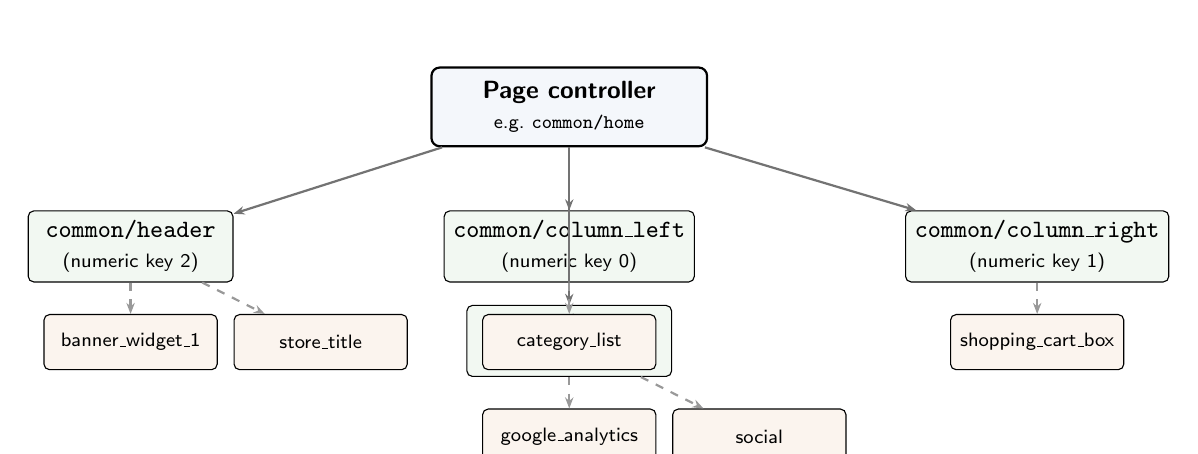
\begin{tikzpicture}[
  parent/.style={draw, rounded corners=3pt, minimum width=3.5cm, minimum height=1.0cm, align=center, font=\small\sffamily, fill=nodefill, thick},
  layout/.style={draw, rounded corners=2pt, minimum width=2.6cm, minimum height=0.8cm, align=center, font=\small\sffamily, fill=nodefillgreen},
  widget/.style={draw, rounded corners=2pt, minimum width=2.2cm, minimum height=0.7cm, align=center, font=\scriptsize\sffamily, fill=nodefillalt},
  arr/.style={-{Stealth[length=4pt]}, thick, black!55}
]
  \node[parent] (page) {\textbf{Page controller}\\\scriptsize e.g.\ \texttt{common/home}};

  \node[layout, below left=0.8cm and 2.5cm of page] (header) {\texttt{common/header}\\\scriptsize (numeric key 2)};
  \node[layout, below=0.8cm of page] (cleft) {\texttt{common/column\_left}\\\scriptsize (numeric key 0)};
  \node[layout, below right=0.8cm and 2.5cm of page] (cright) {\texttt{common/column\_right}\\\scriptsize (numeric key 1)};
  \node[layout, below=2.0cm of page] (footer) {\texttt{common/footer}\\\scriptsize (numeric key 3)};

  \node[widget, below=0.4cm of header] (w1) {banner\_widget\_1};
  \node[widget, right=0.2cm of w1] (w2) {store\_title};
  \node[widget, below=0.4cm of cleft] (w3) {category\_list};
  \node[widget, below=0.4cm of cright] (w4) {shopping\_cart\_box};
  \node[widget, below=0.4cm of footer] (w5) {google\_analytics};
  \node[widget, right=0.2cm of w5] (w6) {social};

  \draw[arr] (page) -- (header);
  \draw[arr] (page) -- (cleft);
  \draw[arr] (page) -- (cright);
  \draw[arr] (page) -- (footer);

  \draw[arr, dashed, black!40] (header) -- (w1);
  \draw[arr, dashed, black!40] (header) -- (w2);
  \draw[arr, dashed, black!40] (cleft) -- (w3);
  \draw[arr, dashed, black!40] (cright) -- (w4);
  \draw[arr, dashed, black!40] (footer) -- (w5);
  \draw[arr, dashed, black!40] (footer) -- (w6);
\end{tikzpicture}
\caption{The composite-view tree. The page controller (e.g.\
\texttt{common/home}) is the parent. Layout children (green,
numeric keys) are added via \texttt{addChild()}. Widget children
(orange, string keys) are merged in via \texttt{loadWidgets()}.
Each child's \texttt{index()} runs recursively, calling its own
\texttt{render()}.}
\label{fig:composite-view}
\end{figure}

\subsection{The \texttt{\{\%widget\_name\%\}} Placeholder}

The widget output is inserted into the parent template by
\texttt{str\_replace} \emph{after} the template has been required.
The tokens are emitted by the \texttt{shared/widgets-rows.tpl}
template (and its variants), which iterates
\texttt{\$rows[\$position]} and emits
\texttt{\{\%<widget\_name>\%\}} for each widget.

\begin{lstlisting}[caption={\texttt{shared/widgets-rows.tpl} --- the placeholder emitter (abridged).},label={lst:widgets-rows}]
<?php if (!isset($rows[$position])) $rows[$position] = []; ?>
<?php foreach ($rows[$position] as $row) { ?>
    <?php if (!isset($row['columns'])) continue; ?>
    <div class="row" data-position="<?php echo $position; ?>" nt-editable="1">
    <?php foreach ($row['columns'] as $column) { ?>
        <div class="col" data-column="<?php echo $column['key']; ?>" nt-editable="1">
        <?php if (!isset($column['widgets'])) $column['widgets'] = []; ?>
        <?php foreach ($column['widgets'] as $w) { ?>
            <?php echo '{%' . $w['name'] . '%}'; ?>
        <?php } ?>
        </div>
    <?php } ?>
    </div>
<?php } ?>
\end{lstlisting}

So the template literally contains the string
\texttt{\{\%banner\_widget\_1\%\}} at the position where the
banner widget should appear. \texttt{fetch()}'s step 8 then
replaces that string with the actual rendered banner HTML.

This is the seam where the composite-view pattern meets the
string-substitution pattern: the tree structure (rows, columns,
widgets) is emitted as flat placeholder tokens, and the
substitution happens after the entire template has been
executed.

% ============================================================
\section{The Widget Data-Access Object: NecoWidget}\label{sec:widget-dao}
% ============================================================

\texttt{NecoWidget} (in \texttt{system/helper/widgets.php}, 785
lines) is the widget data-access object. It queries the
\texttt{property} EAV table for widget rows, columns, and
instances, and returns them as a tree.

\subsection{The Widget Storage Model}

Widget instances, rows, and columns are \emph{not} stored in the
\texttt{widget} table (as one might expect). They are stored in
the polymorphic \texttt{property} EAV table, with
\texttt{object\_type} discriminator:

\begin{table}[htbp]
\centering
\caption{Widget storage in the \texttt{property} EAV table.}\label{tab:widget-storage}
\small
\begin{tabularx}{\columnwidth}{llX}
\toprule
\textbf{object\_type} & \textbf{group} & \textbf{What it stores} \\
\midrule
\texttt{widget\_rows} & \texttt{<position>} (e.g.\ \texttt{header}, \texttt{main}, \texttt{column\_left}) & A row of widgets at a layout position. \texttt{key} is the row ID. \texttt{value} is a serialised PHP array of row settings (landing\_page, app, show\_in\_mobile, customer\_session\_mode, conditional\_logic\_*, style, etc.). \\
\texttt{widget\_cols} & \texttt{<position>} & A column within a row. \texttt{key} is the column ID. \texttt{value} is a serialised array of column settings. \\
\texttt{widget}       & (the \texttt{widget} table itself) & A widget instance. \texttt{settings} column is a serialised array of widget settings (route, module, name, autoload, style, ...). \\
\bottomrule
\end{tabularx}
\end{table}

So a single layout position (e.g.\ \texttt{header}) is a tree:
rows (from \texttt{property}) $\to$ columns (from \texttt{property})
$\to$ widgets (from \texttt{widget}). Each level has a serialised
PHP settings blob.

\subsection{The \texttt{LIKE '\%key=value\%'} Query Pattern}

Every filter on widget rows, columns, and instances is implemented
as a \texttt{LIKE} query against the serialised settings string.
For example, to find widget rows that should show on mobile:

\begin{lstlisting}[caption={The \texttt{LIKE '\%key=value\%'} pattern in \texttt{NecoWidget::getRows()}.},label={lst:like-pattern}]
$sql = "SELECT * FROM " . DB_PREFIX . "property p
    WHERE p.store_id = '" . (int)$data['store_id'] . "'
    AND p.object_type = 'widget_rows'
    AND p.`value` LIKE '%landing_page=all%'
       OR p.`value` LIKE '%landing_page=" . $db->escape($data['landing_page']) . "%'
    AND p.`value` LIKE '%app=" . $db->escape($data['app']) . "%'
    AND p.`value` LIKE '%show_in_mobile=on%'
    AND (p.`value` LIKE '%customer_session_mode=logon%'
         OR p.`value` LIKE '%customer_session_mode=any%')
    ORDER BY p.`order` ASC";
\end{lstlisting}

This works because PHP's \texttt{serialize()} produces deterministic
string representations (e.g.\
\texttt{s:13:"show\_in\_mobile";s:1:"1";}). But it has three
consequences:

\begin{itemize}[leftmargin=1.6em,itemsep=2pt]
  \item \textbf{No index can be used.} The \texttt{LIKE '\%...\%'}
        predicate forces a full-table scan on every widget lookup.
        On a page with 5 layout positions, each with 3 rows, each
        with 2 columns, each with 4 widgets, that is
        $5 \times 3 + 5 \times 3 \times 2 + 5 \times 3 \times 2 \times 4 = 165$
        full-table scans.
  \item \textbf{Substring false-positives are possible.} A widget
        named \texttt{'mobile'} would match
        \texttt{LIKE '\%showonmobile\%'} even if
        \texttt{showonmobile} is not actually set. The codebase
        works around this by adding redundant
        \texttt{filter\_<key>} string duplicates of the real
        settings.
  \item \textbf{The boolean is checked by string-presence}, not by
        unserialising and reading the actual value. So
        \texttt{show\_in\_mobile = '0'} (a false value) would still
        match \texttt{LIKE '\%show\_in\_mobile\%'}.
\end{itemize}

\subsection{The \texttt{getRows()} Algorithm}

\texttt{getRows(\$data, \$useCache = true)} is the main method. It
returns a list of rows, each with a \texttt{columns} key (list of
columns, each with a \texttt{widgets} key), plus the merged
\texttt{children} and \texttt{widget} lookup maps.

\begin{enumerate}[leftmargin=1.6em,itemsep=2pt]
  \item \textbf{Cache key construction.} The cache prefix is
        \texttt{"widgets.rows."} followed by the app, landing\_page,
        store\_id, object\_type, object\_id --- all space-separated.
        The cache is bypassed if the admin is logged in.
  \item \textbf{SQL query.} \texttt{SELECT * FROM property p} with
        the \texttt{LIKE '\%...\%'} predicates.
  \item \textbf{Conditional-logic filter.} The row's
        \texttt{conditional\_logic\_when\_route\_contains} is
        exploded on commas. The
        \texttt{conditional\_logic\_action} is \texttt{'show'} or
        \texttt{'hide'}. The row is kept or removed based on
        whether the current route contains any of the condition
        words.
  \item \textbf{Fetch columns.} Calls \texttt{getCols(\$col\_data)}
        for each row, which runs the same algorithm against
        \texttt{object\_type = 'widget\_cols'}.
  \item \textbf{Fetch widgets.} For each widget in each column,
        unserialise \texttt{settings}, apply
        \texttt{customer\_session\_mode} and
        \texttt{conditional\_logic} filters, and if
        \texttt{settings['autoload']} is set:
        \begin{itemize}[itemsep=2pt]
          \item Emit \texttt{loadWidget} event.
          \item \texttt{\$\_children[\$w['name']] = \$settings['route'];}
                (e.g.\ \texttt{'module/banner'}).
          \item \texttt{\$\_widget[\$w['name']] = \$w;} (the raw
                widget row).
        \end{itemize}
  \item \textbf{Cache write-back.}
        \texttt{\$this->cache->set(\$cachedId, \$result->rows,
        \$prefix);}
  \item \textbf{Return} \texttt{\$result->rows}.
\end{enumerate}

\subsection{The Three Filter Dimensions}

Every widget, row, and column is filtered on three dimensions:

\begin{table}[htbp]
\centering
\caption{The three widget filter dimensions.}\label{tab:widget-filters}
\small
\begin{tabularx}{\columnwidth}{lX}
\toprule
\textbf{Dimension} & \textbf{Values and semantics} \\
\midrule
\texttt{customer\_session\_mode} & \texttt{'any'} (default), \texttt{'logon'} (only when customer is logged in), \texttt{'logoff'} (only when logged out). \\
\texttt{show\_in\_*} & \texttt{show\_in\_mobile}, \texttt{show\_in\_tablet}, \texttt{show\_in\_facebook}, \texttt{show\_in\_desktop} --- device-class visibility. Checked against the \texttt{Browser} library's classification. \\
\texttt{conditional\_logic\_*} & \texttt{conditional\_logic\_action} (\texttt{'show'} or \texttt{'hide'}) + \texttt{conditional\_logic\_when\_route\_contains} (comma-separated route words). The literal word \texttt{"any"} always passes. \\
\bottomrule
\end{tabularx}
\end{table}

\subsection{The Per-Object Override}

If the session has \texttt{object\_type} or \texttt{object\_id}
set (used for per-object widget overrides, e.g.\ different widgets
on different product pages), \texttt{loadWidgets()} calls
\texttt{getRows()} again with the object filter, and merges those
rows into the main result. This is how a specific product page can
show a different set of widgets than the default.

% ============================================================
\section{The Asset Manifest: \texttt{deps.php}}\label{sec:assets}
% ============================================================

At boot, \texttt{app/shop/map.php} loads two PHP manifest files
that declare which CSS/JS files apply to which routes:

\begin{itemize}[leftmargin=1.6em,itemsep=2pt]
  \item \texttt{web/assets/theme/choroni/css/deps.php} (177 lines)
  \item \texttt{web/assets/theme/choroni/js/deps.php} (154 lines)
\end{itemize}

\subsection{The Four Asset Manifests}

Each \texttt{deps.php} file populates one of four registry-stored
manifests:

\begin{table}[htbp]
\centering
\caption{The four asset manifests.}\label{tab:asset-manifests}
\footnotesize\sloppy
\begin{tabularx}{\columnwidth}{>{\raggedright\arraybackslash}p{3.0cm}>{\raggedright\arraybackslash}p{4.5cm}X}
\toprule
\textbf{Manifest} & \textbf{Shape} & \textbf{Used for} \\
\midrule
\texttt{js\_assets}         & \texttt{filepath => routes} or \texttt{'*'} & JS files loaded at the bottom of the page (in the footer). \\
\texttt{js\_header\_assets} & same shape & JS files loaded in \texttt{<head>} (e.g.\ modernizr, polyfills). \\
\texttt{jsx\_assets}        & same shape & JS files inlined as \texttt{<script>...</script>} blocks. \\
\texttt{css\_assets}        & \texttt{key => [css, routes]} & CSS files. \\
\bottomrule
\end{tabularx}
\end{table}

\subsection{Route Matching}

At boot, \texttt{map.php} filters the manifest entries by the
current route and pushes matching entries into the per-request
accumulators (\texttt{\$javascripts},
\texttt{\$header\_javascripts}, \texttt{\$scripts},
\texttt{\$styles}). Non-matching entries stay in the manifests and
are later consumed by \texttt{Module::loadDeps(\$route)} when a
module is rendered.

The route matching is exact-string: an entry with
\texttt{routes => ['*']} matches every route; an entry with
\texttt{routes => ['common/home', 'store/product']} matches only
those exact routes.

\subsection{The Module Asset Loading}

Each storefront widget controller extends \texttt{Module}, which
calls \texttt{loadDeps(\$this->moduleRoute)} in its constructor.
\texttt{loadDeps()} iterates the four manifests, matches the
module's route (e.g.\ \texttt{module/banner}), and pushes the
matching entries into the accumulators. Matched entries are
\texttt{unset()} from the manifest so they don't get loaded
twice.

\begin{lstlisting}[caption={\texttt{Module::loadDeps()} --- the module asset loader (abridged).},label={lst:loaddeps}]
public function loadDeps($route) {
    foreach (['js_assets', 'js_header_assets', 'jsx_assets', 'css_assets'] as $manifest_name) {
        $manifest = $this->registry->get($manifest_name) ?: [];
        foreach ($manifest as $key => $entry) {
            $routes = isset($entry['routes']) ? $entry['routes'] : $entry;
            if ($routes === '*' || in_array($route, (array)$routes)) {
                // Push into the appropriate accumulator
                if ($manifest_name === 'js_assets')         $this->javascripts[]      = $key;
                elseif ($manifest_name === 'js_header_assets') $this->header_javascripts[] = $key;
                elseif ($manifest_name === 'jsx_assets')    $this->scripts[]          = file_get_contents($key);
                elseif ($manifest_name === 'css_assets')    $this->styles[$entry['css']['href']] = $entry['css'];
                // Remove from manifest so it doesn't get loaded twice
                unset($manifest[$key]);
            }
        }
        $this->registry->set($manifest_name, $manifest);
    }
}
\end{lstlisting}

% ============================================================
\section{The Six Layout Composers}\label{sec:layout-composers}
% ============================================================

Six storefront common controllers compose the page layout. Each
storefront page controller calls some subset of them as children
via \texttt{addChild()}.

\subsection{\texttt{ControllerCommonHome} --- the home page}

\begin{lstlisting}[caption={\texttt{ControllerCommonHome::index()} --- the home page composition (abridged).},label={lst:home}]
public function index() {
    $this->tracker->track(0, 'home_page');

    // Cache key: html-homepage.<lang>.<hl>.<cc>.<customer_id>.<currency>.<store_id>
    $cacheId = 'html-homepage.' . $this->config->get('config_language_id') . "."
             . $this->request->getQuery('hl') . "." . $this->request->getQuery('cc') . "."
             . $this->customer->getId() . "." . $this->config->get('config_currency') . "."
             . (int) $this->config->get('config_store_id');

    if (!$this->user->isLogged()) {
        $cached = $this->cache->get($cacheId);
        if ($cached) { $this->response->setOutput($cached, $this->config->get('config_compression')); return; }
    }

    $this->document->setTitle($this->config->get('config_title_' . $this->config->get('config_language_id')));
    $this->document->setDescription(
        $this->config->get('config_meta_description_' . $this->config->get('config_language_id'))
    );

    $this->session->set('landing_page', 'common/home');

    // Load widgets for three positions
    $this->loadWidgets('featuredContent');
    $this->loadWidgets('main');
    $this->loadWidgets('featuredFooter');

    // Add the four layout children
    $this->addChild('common/column_left');
    $this->addChild('common/column_right');
    $this->addChild('common/header');
    $this->addChild('common/footer');

    $this->cacheId = $cacheId;

    // Template resolution: try config_template first, fall back to 'choroni'
    $template = ($this->config->get('default_view_home')) ?: 'common/home.tpl';
    if (file_exists(DIR_TEMPLATE . $this->config->get('config_template') . '/' . $template)) {
        $this->template = $this->config->get('config_template') . '/' . $template;
    } else {
        $this->template = 'choroni/' . $template;
    }

    $this->response->setOutput($this->render(true), $this->config->get('config_compression'));
}
\end{lstlisting}

The cache key includes the language ID, the \texttt{hl} (language
override) and \texttt{cc} (currency override) GET params, the
customer ID, the currency, and the store ID. So cached pages are
language-, currency-, and store-specific. The cache is bypassed
if an admin is logged in.

\subsection{\texttt{ControllerCommonHeader} --- the page header}

The header controller (378 lines) is the most complex of the six.
It:

\begin{enumerate}[leftmargin=1.6em,itemsep=2pt]
  \item Detects IE and redirects to an IE-specific page if needed.
  \item Handles language and currency switching (POST forms).
  \item Bootstraps the admin token (for the visual editor iframe).
  \item Sets the base URL, logo, icon.
  \item Reads document metadata (title, description, keywords).
  \item Builds OpenGraph tags (only if \texttt{\$params['product']}
        or \texttt{\$params['category']} is set --- effectively dead
        code, since no storefront controller passes params to
        \texttt{addChild('common/header')}). This is a noteworthy
        inconsistency between the header's expectations and its
        callers.
  \item Calls \texttt{loadWidgets('header', 'shop', true)}.
  \item Calls \texttt{loadCss()}:
        \begin{itemize}[itemsep=2pt]
          \item Reads the \texttt{theme} table for
                \texttt{theme\_default\_id}.
          \item Reads \texttt{DIR\_CSS/custom-<theme\_id>-choroni.css}
                if it exists (the generated CSS file from
                \texttt{theme\_style} overrides).
          \item Appends to \texttt{\$this->data['css']}.
        \end{itemize}
  \item Calls \texttt{loadJs()}:
        \begin{itemize}[itemsep=2pt]
          \item Concatenates \texttt{\$header\_javascripts} if
                \texttt{config\_render\_js\_in\_file} is on.
        \end{itemize}
  \item Sets 30+ data keys (logo, title, description, keywords,
        styles, scripts, css, base, icon, links, breadcrumbs,
        search URL, cart URL, wishlist URL, etc.).
  \item Sets \texttt{\$this->id = 'header'}.
  \item Sets template to \texttt{choroni/common/header.tpl}.
  \item Calls \texttt{\$this->render()}.
\end{enumerate}

\subsection{\texttt{ControllerCommonFooter} --- the page footer}

The footer controller:

\begin{enumerate}[leftmargin=1.6em,itemsep=2pt]
  \item Loads the footer language file (\texttt{text\_powered\_by}).
  \item Bucketises the inline scripts into 4 buckets:
        \begin{itemize}[itemsep=2pt]
          \item \texttt{\$this->data['scripts\_ domready']} ---
                jQuery \texttt{\$(function()\{...\})} blocks.
          \item \texttt{\$this->data['scripts\_load']} ---
                \texttt{\$(window).load(...)} blocks.
          \item \texttt{\$this->data['scripts\_unload']} ---
                \texttt{\$(window).unload(...)} blocks.
          \item \texttt{\$this->data['scripts\_plain']} ---
                plain JS (no wrapper).
        \end{itemize}
  \item Calls \texttt{loadWidgets('footer')}.
  \item Calls \texttt{loadCss()}:
        \begin{itemize}[itemsep=2pt]
          \item Route-specific CSS (\texttt{commonfooter.css}).
          \item Per-widget CSS (from each widget's
                \texttt{settings['style']}).
          \item Minification via \texttt{NecoTool::minify()}.
        \end{itemize}
  \item Calls \texttt{loadJs()}:
        \begin{itemize}[itemsep=2pt]
          \item Route-specific JS.
          \item If \texttt{config\_render\_js\_in\_file},
                concatenates all \texttt{\$javascripts} into the
                \texttt{domready} bucket.
        \end{itemize}
  \item Builds 4 \texttt{<script>} blocks (one per bucket).
  \item Sets \texttt{\$this->id = 'footer'}.
  \item Sets template to \texttt{choroni/common/footer.tpl}.
  \item Calls \texttt{\$this->render()}.
\end{enumerate}

\subsection{\texttt{ControllerCommonColumnLeft} / \texttt{ColumnRight}}

Both are minimal. They call \texttt{loadWidgets('column\_left')}
(or \texttt{column\_right}), set the template to
\texttt{choroni/common/column\_left.tpl} (or
\texttt{column\_right.tpl}), and call \texttt{render()}. If no
widgets are assigned to the position, the controller does nothing
(\texttt{\$this->output} stays null), and the parent template's
\texttt{<?php if (\$column\_left) \{ ... \} ?>} check hides the
column.

\subsection{\texttt{ControllerCommonMaintenance}}

Renders the maintenance page. The \texttt{check()} method is the
pre-action: if \texttt{config\_maintenance} is on AND the visitor
is not an admin, it returns \texttt{\$this->forward('common/maintenance')}
which replaces the main action.

% ============================================================
\section{The Theme: \texttt{choroni}}\label{sec:theme}
% ============================================================

The only theme shipped. The whole \texttt{app/shop/view/theme/}
directory contains exactly one subfolder: \texttt{choroni/}.

\subsection{Folder Structure}

\begin{figure}[htbp]
\centering
\resizebox{\columnwidth}{!}{%
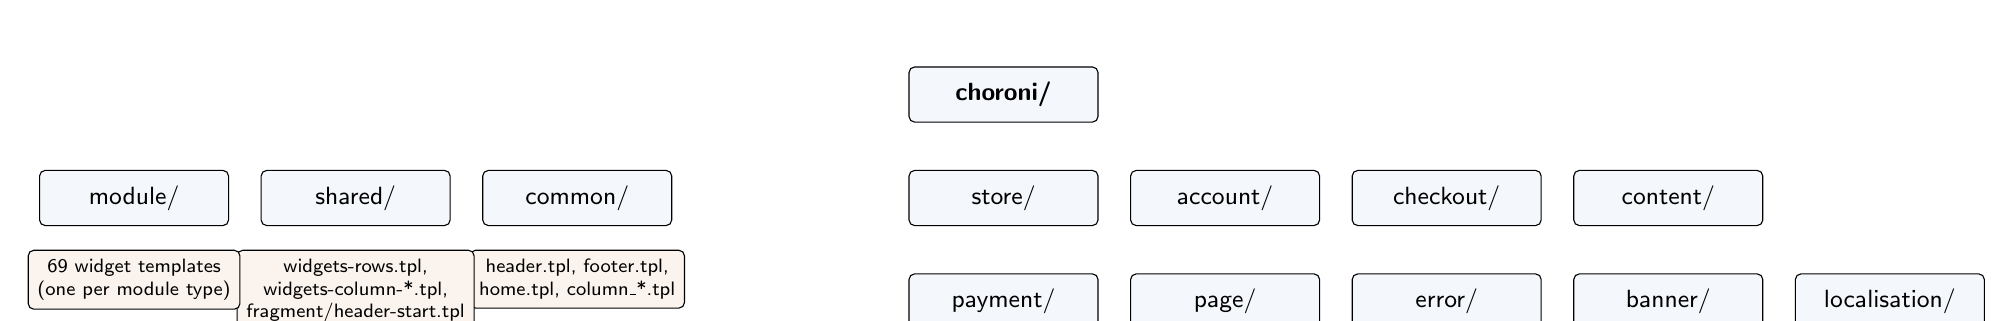
\begin{tikzpicture}[
  dir/.style={draw, rounded corners=2pt, minimum width=2.4cm, minimum height=0.7cm, align=center, font=\small\sffamily, fill=nodefill},
  file/.style={draw, rounded corners=2pt, minimum width=2.4cm, minimum height=0.7cm, align=center, font=\scriptsize\sffamily, fill=nodefillalt},
]
  \node[dir] (root) {\textbf{choroni/}};
  \node[dir, below left=0.6cm and 3.0cm of root] (common) {common/};
  \node[dir, left=0.4cm of common] (shared) {shared/};
  \node[dir, left=0.4cm of shared] (module) {module/};
  \node[dir, below=0.6cm of root] (store) {store/};
  \node[dir, right=0.4cm of store] (account) {account/};
  \node[dir, right=0.4cm of account] (checkout) {checkout/};
  \node[dir, right=0.4cm of checkout] (content) {content/};
  \node[dir, below=0.6cm of store] (payment) {payment/};
  \node[dir, right=0.4cm of payment] (page) {page/};
  \node[dir, right=0.4cm of page] (error) {error/};
  \node[dir, right=0.4cm of error] (banner) {banner/};
  \node[dir, right=0.4cm of banner] (local) {localisation/};

  \node[file, below=0.3cm of common] (htpl) {header.tpl, footer.tpl,\\home.tpl, column\_*.tpl};
  \node[file, below=0.3cm of shared] (stpl) {widgets-rows.tpl,\\widgets-column-*.tpl,\\fragment/header-start.tpl};
  \node[file, below=0.3cm of module] (mtpl) {69 widget templates\\(one per module type)};
\end{tikzpicture}%
}
\caption{The \texttt{choroni} theme folder structure (14 top-level
folders). \texttt{common/} holds the layout templates;
\texttt{shared/} holds the fragments included by every template;
\texttt{module/} holds one template per widget type; the rest
hold per-controller templates.}
\label{fig:theme-tree}
\end{figure}

\subsection{The \texttt{\$tpl} Inheritance Mechanism}

Every template starts with this line:

\begin{lstlisting}[caption={The \texttt{\$tpl} inheritance mechanism.},label={lst:tpl-inherit}]
<?php $tpl = is_dir(DIR_TEMPLATE. $this->config->get('config_template') ."/shared") ? $this->config->get('config_template') : "choroni"; ?>
\end{lstlisting}

This means: if the active theme has a \texttt{/shared} folder, use
that theme's name for \texttt{include()} paths; otherwise fall back
to \texttt{'choroni'}. So a child theme can override e.g.\
\texttt{common/home.tpl} while still inheriting all the
\texttt{shared/} fragments from \texttt{choroni}. The
\texttt{include(DIR\_TEMPLATE. \$tpl ."/shared/widgets-rows.tpl")}
calls in every template use this \texttt{\$tpl} variable.

\subsection{The Shared Fragments}

The \texttt{shared/} folder contains fragments included by every
template. The most important:

\subsubsection{\texttt{shared/fragment/header-start.tpl} (319 lines)}

Included once at the end of \texttt{<head>}. Emits:

\begin{itemize}[leftmargin=1.6em,itemsep=2pt]
  \item A \texttt{<link rel="dns-prefetch" href="www.necoyoad.com">}
        (hard-coded).
  \item A \texttt{<style>} block defining \texttt{:before} content
        for three sticker classes (\texttt{.oferta}, \texttt{.nuevo},
        \texttt{.descuento} --- Spanish for ``offer'', ``new'',
        ``discount'').
  \item All \texttt{\$header\_javascripts} as
        \texttt{<script src="...">} tags.
  \item The inline \texttt{\$scripts} block.
  \item A large inline \texttt{<script>} defining:
        \begin{itemize}[itemsep=2pt]
          \item \texttt{window.I18n} --- a frozen JS object with
                translation strings (addToCart, goToCart, accept,
                cancel, form warnings, etc.).
          \item \texttt{window.Context.User} --- the current
                customer's name and \texttt{isLogged} flag.
          \item \texttt{window.Context.Product} --- the current
                product ID (only set on product pages).
          \item \texttt{window.Constants} --- paths (CSS\_PATH,
                JS\_PATH, IMAGES\_PATH, THEMECSS\_PATH, etc.).
          \item \texttt{window.Requests.QUICK\_VIEW} --- the URL
                for the product quick-view AJAX endpoint.
          \item \texttt{window.Mq} --- media-query match flags
                (small, smallUp, mediumUp, medium, smallToMedium,
                large, largeUp).
        \end{itemize}
  \item A conditional-compilation IE shim.
  \item A \texttt{requestAnimationFrame} polyfill.
  \item A \texttt{popupWindow()} helper.
  \item An async style/script loader (\texttt{fetchStyle},
        \texttt{fetchScript}, \texttt{appendToHead}) --- implements
        the ``critical CSS'' pattern: stylesheets loaded with
        \texttt{media="only x"} are upgraded to
        \texttt{media="screen"} after page load.
\end{itemize}

\subsubsection{\texttt{shared/fragment/footer-start.tpl} (29 lines)}

Included at the end of \texttt{<body>}. Emits:

\begin{itemize}[leftmargin=1.6em,itemsep=2pt]
  \item All \texttt{\$javascripts} as \texttt{<script src="...">} tags.
  \item The inline \texttt{\$scripts} string (the 4-bucket bundle).
  \item Defers remaining \texttt{\$styles} --- they're appended to
        \texttt{<head>} via jQuery on DOM ready (the ``load CSS
        without blocking'' pattern).
  \item Defers remaining \texttt{\$css}.
  \item Calls \texttt{\$().UItoTop();} --- a ``back to top''
        button plugin.
\end{itemize}

\subsubsection{\texttt{shared/widget-head.tpl} (63 lines)}

The wrapper around every widget's content. Opens an \texttt{<li>}
with the widget's metadata as \texttt{data-*} attributes --- used
by the visual theme editor.

\begin{lstlisting}[caption={\texttt{shared/widget-head.tpl} --- the widget wrapper (abridged).},label={lst:widget-head}]
<?php
if (!isset($settings['module']) || empty($settings['module']))
    throw new Exception("FATAL ERROR: The index module is not set for ". $settings['route']);
echo '<li '.
    'data-necotienda_module="'. $settings['module'] .'" '.
    'data-landing_page="'. str_replace('landing_page=', '', $settings['landing_page']) .'" '.
    'data-widget="'. $widgetName .'" '.
    'nt-editable="1" '.
    'movable="1" '.
    'removable="1" '.
    'configurable="1" '.
    'class="box '. $settings['module'] .'-widget'.
        (isset($settings['class']) ? ' '.$settings['class'] : '') .
    '" '.
    'id="'. $widgetName .'" '.
    '>';
?>
\end{lstlisting}

So every widget is wrapped in an \texttt{<li class="box
<module>-widget" id="<widgetName>" data-widget="<widgetName>"
data-necotienda\_module="<module>" nt-editable="1" movable="1"
removable="1" configurable="1">}. The \texttt{nt-editable="1"},
\texttt{movable="1"}, \texttt{removable="1"},
\texttt{configurable="1"} attributes are the visual editor's hooks.

If \texttt{\$settings['module']} is not set, the template throws a
fatal exception --- this is a hard contract: every widget must
declare its module name in settings.

\subsection{The Module Templates}

The \texttt{module/} folder contains one \texttt{.tpl} file per
widget type. Each is a small PHP template that renders the
widget's HTML. For example, \texttt{module/category\_list.tpl}
iterates the categories and emits \texttt{<li>} entries with
links; \texttt{module/store\_logo.tpl} emits an
\texttt{<img src="...">} with the store's logo.

Many modules have multiple templates (e.g.\
\texttt{category\_list.tpl},
\texttt{category\_list\_default.tpl}, \texttt{category\_list\_grid.tpl})
for different display modes. The widget's \texttt{settings['view']}
selects which template is used.

% ============================================================
\section{Device Detection and Theme Switching}\label{sec:device}
% ============================================================

The \texttt{Browser} library (\texttt{system/library/browser.php})
classifies the request into four device classes:
\texttt{isMobile()}, \texttt{isTablet()}, \texttt{isFacebook()}
(in-app browser), and the implicit ``desktop'' (none of the
above). Each class can either redirect to a separate URL or swap
\texttt{config\_template} to a per-device theme.

\begin{lstlisting}[caption={The mobile template switching code in \texttt{app/shop/map.php}.},label={lst:mobile-switch}]
$loader->library('browser');
$browser = new Browser;
if ($browser->isMobile()) {
    if ($config->get('config_redirect_when_mobile')
        && str_replace('/web','',HTTP_HOME) !== $config->get('config_mobile_url')) {
        if (!headers_sent()) {
            header('Location: ' . $config->get('config_mobile_url'));
            exit;
        } else {
            echo "<script> window.location = '". $config->get('config_mobile_url') ."'; </script>";
        }
    } else {
        $config->set('config_template', $config->get('config_mobile_template'));
    }
} elseif ($browser->isTablet()) {
    if ($config->get('config_redirect_when_tablet')
        && str_replace('/web','',HTTP_HOME) !== $config->get('config_tablet_url')) {
        header('Location: ' . $config->get('config_tablet_url'));
        exit;
    } else {
        $config->set('config_template', $config->get('config_tablet_template'));
    }
} elseif ($browser->isFacebook()) {
    if ($config->get('config_redirect_when_facebbok')   // typo in source: 'facebbok'
        && str_replace('/web','',HTTP_HOME) !== $config->get('config_facebook_url')) {
        header('Location: ' . $config->get('config_facebook_url'));
        exit;
    } else {
        $config->set('config_template', $config->get('config_facebook_theme'));
    }
}
\end{lstlisting}

Three device classes, two strategies per class:
\begin{enumerate}[leftmargin=1.6em,itemsep=2pt]
  \item \textbf{Redirect to a separate URL} (\texttt{config\_<class>\_url})
        if \texttt{config\_redirect\_when\_<class>} is on AND the
        current URL isn't already that URL.
  \item \textbf{Otherwise swap the template} (\texttt{config\_<class>\_template}
        for mobile/tablet, \texttt{config\_facebook\_theme} for
        Facebook).
\end{enumerate}

The template swap is just a \texttt{Config::set('config\_template', ...)}
call --- every subsequent file-existence check
(\texttt{file\_exists(DIR\_TEMPLATE . \$config->get('config\_template') . '/...')})
sees the new template name. If the mobile template folder is
missing files, the universal fallback is \texttt{'choroni'} (because
every \texttt{if file\_exists} has an \texttt{else} branch that
uses \texttt{'choroni'}).

\subsection{The Template-Preview Override}

\begin{lstlisting}[caption={The template-preview override in \texttt{app/shop/map.php}.},label={lst:template-preview}]
if (!empty($_GET['template']) && file_exists(DIR_TEMPLATE . $_GET['template'] . '/common/header.tpl')) {
    $config->set('config_template', $_GET['template']);
}
\end{lstlisting}

Passing \texttt{?template=<name>} in the URL swaps the theme for
that request, as long as the theme folder has a
\texttt{common/header.tpl} (the existence check uses
\texttt{header.tpl} as the ``is this a real theme?'' sentinel).
This is used by the admin's ``preview theme'' functionality.

\subsection{Admin Force-Override GET Params}

For testing, an admin can pass \texttt{?force\_mobile=1},
\texttt{?force\_tablet=1}, \texttt{?force\_facebook=1}, or
\texttt{?force\_customer\_session=1} to override the device
classification and customer-session mode. These are checked in
\texttt{Controller::loadWidgets()}.

% ============================================================
\section{The Visual Theme Editor and \texttt{theme\_style}}\label{sec:visual-editor}
% ============================================================

Necoyoad includes a visual theme editor (accessible from the
admin) that lets a non-technical user rearrange widgets, edit
their settings, and write CSS overrides at the
selector/property/value granularity --- all without editing any
files.

\subsection{The \texttt{nt-editable} Hook}

Every \texttt{<div>} that the visual editor can manipulate has
\texttt{nt-editable="1"} (or just \texttt{nt-editable}) as an HTML
attribute. The editor's JS scans the DOM for these attributes and
attaches click/drag handlers. The companion attributes
\texttt{data-row}, \texttt{data-column}, \texttt{data-widget},
\texttt{data-position}, \texttt{data-necotienda\_module} carry
the metadata needed to identify which widget is being edited.

The \texttt{shared/widget-head.tpl} wrapper (Listing~\ref{lst:widget-head})
emits all of these. The \texttt{shared/widgets-rows.tpl} template
emits them on the row and column wrappers. So every level of the
widget tree is editable.

\subsection{The Inline CSS Markers}

When a widget's settings include a \texttt{style} key (raw CSS for
that widget), \texttt{Controller::loadWidgets()} wraps the CSS in
comment markers before appending it to \texttt{\$this->css}:

\begin{lstlisting}[caption={The inline CSS markers (used by the visual editor).},label={lst:css-markers}]
if (isset($settings['style'])) {
    $this->css .= "/**{$row['key']}**/"
                . NecoTool::minify($settings['style'])
                . "/**/{$row['key']}**/";
}
\end{lstlisting}

The \texttt{/**key**/ ... /**/key**/} markers let the visual editor
find and replace a specific widget's CSS block without touching
the others. When the editor saves a new style for widget
\texttt{banner\_widget\_1}, it does a regex replace on
\texttt{/**banner\_widget\_1**/.../**/banner\_widget\_1**/} in the
CSS string.

\subsection{The \texttt{theme\_style} Table}

The \texttt{theme\_style} table stores CSS-rule overrides at the
selector/property/value granularity:

\begin{table}[htbp]
\centering
\caption{The \texttt{theme\_style} table schema.}\label{tab:theme-style}
\small
\begin{tabularx}{\columnwidth}{llX}
\toprule
\textbf{Column} & \textbf{Type} & \textbf{Purpose} \\
\midrule
\texttt{theme\_style\_id} & \texttt{INT} & Primary key. \\
\texttt{theme\_id}        & \texttt{INT} & The theme this override belongs to. \\
\texttt{selector}         & \texttt{VARCHAR(250)} & The CSS selector (e.g.\ \texttt{.product-list .price}). \\
\texttt{property}         & \texttt{VARCHAR(250)} & The CSS property (e.g.\ \texttt{color}). \\
\texttt{value}            & \texttt{VARCHAR(250)} & The CSS value (e.g.\ \texttt{\#ff0000}). \\
\bottomrule
\end{tabularx}
\end{table}

\subsection{The CSS Generator}

The admin's \texttt{style/theme.php} controller has a \texttt{save()}
method that reads all \texttt{theme\_style} rows for the current
theme and generates a CSS file:

\begin{lstlisting}[caption={\texttt{ModelStyleTheme::saveStyle()} --- the CSS generator (abridged).},label={lst:css-gen}]
public function saveStyle($theme_id, $styles) {
    $css = '';
    $current_selector = null;
    foreach ($styles as $style) {
        if ($style['selector'] !== $current_selector) {
            if ($current_selector !== null) $css .= "}\n";
            $css .= $style['selector'] . " {\n";
            $current_selector = $style['selector'];
        }
        $css .= "  " . $style['property'] . ": " . $style['value'] . ";\n";
    }
    if ($current_selector !== null) $css .= "}\n";

    // Write to a custom CSS file that the header controller loads
    $file = DIR_CSS . "custom-{$theme_id}-" . $config_template . ".css";
    file_put_contents($file, $css);
    return $file;
}
\end{lstlisting}

The generated CSS file (\texttt{custom-<theme\_id>-choroni.css})
is read by \texttt{ControllerCommonHeader::loadCss()} and
appended to \texttt{\$this->data['css']} (the inline CSS string).
So every page load includes the admin-defined CSS overrides,
generated from the \texttt{theme\_style} table.

% ============================================================
\section{Hooks and Events in the Rendering Pipeline}\label{sec:hooks-seams}
% ============================================================

The rendering pipeline fires 18 Hooks (short-circuit, can replace
the return value) and 10 Events (notification, no short-circuit)
at well-defined points. This is the seam where modules extend
the presentation layer.

\subsection{Hook Emit Points (Short-Circuit)}

\begin{table}[htbp]
\centering
\caption{The 18 Hook emit points in the rendering pipeline.}\label{tab:hooks}
\footnotesize\sloppy
\begin{tabularx}{\columnwidth}{llX}
\toprule
\textbf{Hook} & \textbf{Fired by} & \textbf{Effect of truthy return} \\
\midrule
\texttt{render}        & \texttt{Controller::render()}    & Bypasses the entire render; the truthy value is returned as the HTML. \\
\texttt{fetch}         & \texttt{Controller::fetch()}     & Bypasses the template execution; the truthy value is returned as the HTML. \\
\texttt{loadWidgets}   & \texttt{Controller::loadWidgets()} & Bypasses the widget query; the truthy value is used as the widget tree. \\
\texttt{loadAssets}    & \texttt{Controller::loadAssets()} & Bypasses the asset file discovery. \\
\texttt{redirect}      & \texttt{Controller::redirect()}  & Bypasses the \texttt{header('Location:')} call. \\
\texttt{index}         & \texttt{ControllerModuleModuleController::index()} & Bypasses the widget's index method. \\
\texttt{async}         & \texttt{ControllerModuleModuleController::async()} & Bypasses the widget's async method. \\
\texttt{csspath}       & \texttt{Controller::loadAssets()} & Rewrites the CSS HTTP path. \\
\texttt{cssfolder}     & \texttt{Controller::loadAssets()} & Rewrites the CSS filesystem path. \\
\texttt{jspath}        & \texttt{Controller::loadAssets()} & Rewrites the JS HTTP path. \\
\texttt{jsfolder}      & \texttt{Controller::loadAssets()} & Rewrites the JS filesystem path. \\
\texttt{loadcss}       & \texttt{ControllerCommonHeader::loadCss()} & Rewrites the CSS accumulator. \\
\texttt{loadstyles}    & \texttt{Controller::loadAssets()} & Rewrites the \texttt{\$styles} array. \\
\texttt{loadjavascripts} & \texttt{Controller::loadAssets()} & Rewrites the \texttt{\$javascripts} array. \\
\texttt{processcss}    & \texttt{startup.php}             & Rewrites the CSS after processing. \\
\texttt{rowcss}        & \texttt{Controller::loadWidgets()} & Rewrites the per-row CSS. \\
\texttt{columncss}     & \texttt{Controller::loadWidgets()} & Rewrites the per-column CSS. \\
\texttt{widget:settings} & widget controllers            & Rewrites a widget's settings before rendering. \\
\texttt{module:settings} & module controllers            & Rewrites a module's settings before rendering. \\
\bottomrule
\end{tabularx}
\end{table}

\subsection{Event Emit Points (Notification)}

\begin{table}[htbp]
\centering
\caption{The 10 Event emit points in the rendering pipeline.}\label{tab:events}
\small
\begin{tabularx}{\columnwidth}{llX}
\toprule
\textbf{Event} & \textbf{Fired by} & \textbf{Payload} \\
\midrule
\texttt{addChild}        & \texttt{Controller::addChild()}      & (\$child, \$params) \\
\texttt{beforeLoad}      & \texttt{Controller::render()} child loop & (\$action, \$controller, \$params) \\
\texttt{afterLoad}       & \texttt{Controller::render()} child loop & (\$controller) \\
\texttt{beforeRender}    & \texttt{Controller::render()}        & (\$template\_path) \\
\texttt{afterRender}     & \texttt{Controller::render()}        & (\$rendered\_html) \\
\texttt{renderWidget}    & \texttt{Controller::fetch()}         & (\$widget\_name) \\
\texttt{beforeLoadWidget}& \texttt{Controller::loadWidgets()}   & (\$params) \\
\texttt{loadWidget}      & \texttt{NecoWidget::getRows()}       & (\$widget) \\
\texttt{dispatch}        & \texttt{Front::dispatch()}           & (\$action) \\
\texttt{registry:update} & \texttt{Registry::set()}             & (\$key, \$value) \\
\bottomrule
\end{tabularx}
\end{table}

\subsection{The Dual Emission Pattern}

Many call sites fire both a Hook and an Event for the same
occurrence. For example, \texttt{Controller::redirect()} runs the
\texttt{redirect} hook (short-circuit) AND emits the
\texttt{redirect} event. This dual emission is the pattern across
the codebase: Hooks are for modules that want to \emph{change}
the behaviour; Events are for modules that want to \emph{observe}
it.

% ============================================================
\section{The Full Rendering Pipeline Trace}\label{sec:trace}
% ============================================================

This trace walks through the rendering of the home page
(\texttt{common/home}) for a non-logged-in customer on a desktop
browser, with \texttt{config\_seo\_url} on,
\texttt{config\_render\_css\_in\_file} on,
\texttt{config\_minified\_html} off, and the \texttt{choroni}
theme active.

\subsection{Phase 1 --- Entry and Bootstrap (Steps 1--5)}

\begin{enumerate}[leftmargin=1.6em,itemsep=2pt]
  \item \texttt{web/index.php} detects the store (URL path folder
        match), sets \texttt{STORE\_ID}, \texttt{DIR\_APPLICATION},
        etc., includes \texttt{app/shop/config.php} and
        \texttt{app/shop/map.php}.
  \item \texttt{app/shop/map.php} boots the registry, loads
        settings from \texttt{setting} table, detects
        language/currency, loads libraries, detects device
        (desktop $\to$ no template swap), loads
        \texttt{deps.php} for the active theme (populates
        \texttt{\$js\_assets}, \texttt{\$js\_header\_assets},
        \texttt{\$jsx\_assets}, \texttt{\$css\_assets}), filters
        the manifest by the current route (\texttt{common/home})
        and pushes matching entries into \texttt{\$javascripts},
        \texttt{\$header\_javascripts}, \texttt{\$styles},
        \texttt{\$scripts}.
  \item \texttt{web/index.php} builds a \texttt{Front} controller,
        adds pre-actions (\texttt{common/maintenance/check},
        \texttt{common/seo\_url}), and calls
        \texttt{\$controller->dispatch(new Action('common/home'),
        new Action('error/not\_found'))}.
  \item \texttt{Front::dispatch()} runs the pre-actions:
        \begin{itemize}[itemsep=2pt]
          \item \texttt{common/maintenance/check}: \texttt{config\_maintenance}
                is off, so no short-circuit.
          \item \texttt{common/seo\_url}: parses
                \texttt{?\_route\_=} (or \texttt{?r=}) and resolves
                SEO URLs to route+params via the \texttt{url\_alias}
                table.
        \end{itemize}
  \item The main action (\texttt{common/home}) is executed.
\end{enumerate}

\subsection{Phase 2 --- Controller Setup (Steps 6--11)}

\begin{enumerate}[leftmargin=1.6em,itemsep=2pt]
  \setcounter{enumi}{5}
  \item \texttt{\$this->tracker->track(0, 'home\_page')} ---
        inserts a row in the \texttt{tracker} table.
  \item Cache key construction: \texttt{'html-homepage.<lang\_id>...'}
        --- the full key includes lang\_id, hl, cc, customer\_id,
        currency, and store\_id.
  \item \texttt{\$this->cache->get(\$cacheId)} --- cache miss
        (first visit).
  \item \texttt{\$this->document->setTitle(...)} --- sets the page
        title from the per-language setting.
  \item \texttt{\$this->session->set('landing\_page', 'common/home')}
        --- stores the current route in the session (used by
        NecoWidget for landing\_page filtering).
  \item \texttt{\$this->loadWidgets('featuredContent')} ---
        loads widgets for the \texttt{featuredContent} position.
        This calls \texttt{NecoWidget::getRows()} which queries
        \texttt{property} (for rows) $\to$ \texttt{property} (for
        columns) $\to$ \texttt{widget} (for widgets). The widgets'
        children/routes are merged into \texttt{\$this->children}
        and \texttt{\$this->widget}. The rows are stored in
        \texttt{\$this->data['rows']['featuredContent']}.
\end{enumerate}

\subsection{Phase 3 --- Widget Loading and Child Composition (Steps 12--19)}

\begin{enumerate}[leftmargin=1.6em,itemsep=2pt]
  \setcounter{enumi}{11}
  \item \texttt{\$this->loadWidgets('main')} --- same for the
        \texttt{main} position (the center column).
  \item \texttt{\$this->loadWidgets('featuredFooter')} --- same
        for the \texttt{featuredFooter} position.
  \item \texttt{\$this->addChild('common/column\_left')} ---
        pushes \texttt{'common/column\_left'} onto
        \texttt{\$this->children} with numeric key 0.
  \item \texttt{\$this->addChild('common/column\_right')} ---
        numeric key 1.
  \item \texttt{\$this->addChild('common/header')} --- numeric
        key 2.
  \item \texttt{\$this->addChild('common/footer')} --- numeric
        key 3.
  \item \texttt{\$this->cacheId = \$cacheId} (only if admin is
        NOT logged in --- enables cache write-back).
  \item Template resolution: \texttt{\$this->template =
        'choroni/common/home.tpl'} (since
        \texttt{config\_template} is \texttt{'choroni'} and the
        file exists).
\end{enumerate}

\subsection{Phase 4 --- Render (Steps 20--28)}

\begin{enumerate}[leftmargin=1.6em,itemsep=2pt]
  \setcounter{enumi}{19}
  \item \texttt{\$this->response->setOutput(\$this->render(true),
        ...)} --- enters \texttt{Controller::render(true)}.
  \item \texttt{runHook("render", \$this, true)} --- no handlers
        registered, returns null. Continue.
  \item \texttt{\$device = '.pc'} (desktop browser).
        \texttt{\$this->cacheId .= '.pc'}.
  \item \texttt{\$customerLogged = 0} (not logged in).
        \texttt{\$this->cacheId .= '0'}.
  \item \texttt{\$cached = \$cache->get(\$this->cacheId, ...)}
        --- cache miss (first visit).
  \item Cache miss $\to$ asset loading:
        \begin{itemize}[itemsep=2pt]
          \item \texttt{loadAssets('ControllerCommonHome', 'shop')}
                --- strips \texttt{controller} from classname $\to$
                \texttt{'commonhome'}. Looks for
                \texttt{web/assets/theme/choroni/css/commonhome.css}
                --- doesn't exist, so no CSS loaded. Same for JS.
          \item \texttt{loadAssets('common/home', 'shop')} ---
                strips slashes $\to$ \texttt{'commonhome'} (same
                as above, deduplicated by \texttt{\$assetLoaded}).
        \end{itemize}
  \item Child loop (in FIFO order):
        \begin{itemize}[itemsep=2pt]
          \item \textbf{Child 0: \texttt{'common/column\_left'}}
                --- \texttt{new Action('common/column\_left')} $\to$
                file \texttt{app/shop/controller/common/column\_left.php},
                class \texttt{ControllerCommonColumnLeft}, method
                \texttt{index}. \texttt{require\_once}, instantiate,
                call \texttt{\$controller->index(null)}. Inside:
                \texttt{loadWidgets('column\_left')} $\to$ queries
                \texttt{property} + \texttt{widget}. If there are
                widgets, sets template to
                \texttt{choroni/common/column\_left.tpl} and calls
                \texttt{\$this->render()}. If not, does nothing
                (output stays null). Back in the parent:
                \texttt{\$this->data['column\_left'] = \$output}.
          \item \textbf{Child 1: \texttt{'common/column\_right'}} ---
                same pattern,
                \texttt{\$this->data['column\_right'] = \$output}.
          \item \textbf{Child 2: \texttt{'common/header'}} ---
                \texttt{ControllerCommonHeader::index(null)}.
                Inside: IE detection, language/currency switching,
                token bootstrap, base URL, logo/icon, document
                metadata read, OpenGraph (skipped ---
                \texttt{\$params} is null), admin-mode check (no),
                \texttt{loadWidgets('header', 'shop', true)} $\to$
                queries \texttt{property} + \texttt{widget} for the
                \texttt{header} position. \texttt{loadCss()} $\to$
                reads \texttt{theme} table for
                \texttt{theme\_default\_id}, reads
                \texttt{DIR\_CSS/custom-<theme\_id>-choroni.css}
                if it exists, appends to
                \texttt{\$this->data['css']}. \texttt{loadJs()} $\to$
                concatenates \texttt{\$header\_javascripts} if
                \texttt{config\_render\_js\_in\_file}. Sets 30+
                data keys. Sets \texttt{\$this->id = 'header'}.
                Sets template to
                \texttt{choroni/common/header.tpl}. Calls
                \texttt{\$this->render()}. Inside
                \texttt{Controller::render()} (header's own
                render): \texttt{loadAssets('ControllerCommonHeader', 'shop')}
                $\to$ looks for \texttt{commonheader.css} (doesn't
                exist). Child loop: no children (the header
                doesn't \texttt{addChild} anything).
                \texttt{fetch('choroni/common/header.tpl')}.
                Inside \texttt{fetch()}: injects magic services,
                \texttt{extract(\$this->data)}, \texttt{require header.tpl}.
                The template emits \texttt{<!doctype html>},
                \texttt{<head>} with meta + styles + inline CSS +
                \texttt{header-start.tpl} (which emits the I18n
                script + polyfills), \texttt{<body>},
                \texttt{\#mainContainer}, \texttt{\#headerContainer},
                \texttt{\#header} div with \texttt{widgets-rows.tpl}
                (which iterates \texttt{\$rows['header']} and emits
                \texttt{\{\%widget\_name\%\}} placeholders).
                Post-processing: strip comments, collapse
                whitespace. \texttt{applyFilters("render", \$content)}
                --- no filters registered. Returns the HTML. Back
                in the parent: \texttt{\$this->data['header'] = \$output}.
          \item \textbf{Child 3: \texttt{'common/footer'}} ---
                \texttt{ControllerCommonFooter::index(null)}.
                Inside: language load, \texttt{text\_powered\_by},
                script bucketing (4 buckets),
                \texttt{loadWidgets('footer')} $\to$ queries for
                \texttt{footer} widgets. \texttt{loadCss()} $\to$
                route-specific CSS + per-widget CSS + minification
                via \texttt{NecoTool::minify()}.
                \texttt{loadJs()} $\to$ route-specific JS. If
                \texttt{config\_render\_js\_in\_file}, concatenates
                all \texttt{\$javascripts} into the function
                bucket. Builds 4 \texttt{<script>} blocks. Sets
                \texttt{\$this->id = 'footer'}. Template
                \texttt{choroni/common/footer.tpl}. Calls
                \texttt{\$this->render()}. Inside \texttt{fetch()}:
                the footer template emits \texttt{\#footerContainer},
                \texttt{\#footer} div with
                \texttt{widgets-rows.tpl}, \texttt{\#copyright},
                \texttt{footer-start.tpl} (which emits all
                \texttt{<script src>} tags + the 4-bucket
                \texttt{<script>} blocks + deferred
                \texttt{<link>} and \texttt{<style>} injection +
                \texttt{\$().UItoTop();}), then closes
                \texttt{\#mainContainer}, \texttt{<body>},
                \texttt{<html>}. Back in the parent:
                \texttt{\$this->data['footer'] = \$output}.
          \item \textbf{Widget children (string keys)} --- these
                were merged in during
                \texttt{loadWidgets('featuredContent')},
                \texttt{loadWidgets('main')},
                \texttt{loadWidgets('featuredFooter')}, and
                possibly \texttt{loadWidgets('header')} /
                \texttt{loadWidgets('footer')}. For each widget
                child:
                \begin{itemize}[itemsep=2pt]
                  \item \texttt{new Action(\$settings['route'])}
                        $\to$ e.g.\ \texttt{'module/banner'} $\to$
                        \texttt{app/shop/controller/module/banner.php},
                        class \texttt{ControllerModuleBanner},
                        method \texttt{index}.
                  \item \texttt{require\_once}, instantiate, call
                        \texttt{\$controller->index(\$widget)} where
                        \texttt{\$widget} is the widget row from
                        \texttt{\$this->widget[\$key]}.
                  \item Inside
                        \texttt{ControllerModuleModuleController::index(\$widget, false)}:
                        \texttt{init()} $\to$
                        \texttt{ControllerModuleBanner::init()}
                        registers the \texttt{module:settings}
                        filter. \texttt{runHook("index", \$this)}
                        --- no handlers.
                        \texttt{trigger('moduleLoad', ...)} ---
                        event. Load language
                        \texttt{module/banner}. Unserialise
                        \texttt{\$widget['settings']}. Apply
                        defaults. Minify \texttt{settings['style']}
                        if set, append to \texttt{\$this->css}.
                        \texttt{loadDeps('module/banner/default')}
                        $\to$ filters the \texttt{deps.php}
                        manifests for matching routes. Template
                        resolution: \texttt{choroni/module/banner.tpl}
                        (doesn't exist) $\to$ falls back to...
                        the banner module overrides the template
                        in its \texttt{module:settings} filter
                        (sets it to
                        \texttt{choroni/banner/<jquery\_plugin>.tpl}).
                        So the template becomes e.g.\
                        \texttt{choroni/banner/nivo-slider.tpl}.
                        Apply \texttt{module:settings} filter $\to$
                        \texttt{ControllerModuleBanner::init()}'s
                        filter runs: loads the banner by
                        \texttt{banner\_id}, loads the banner
                        items, loads per-item widgets (recursive
                        \texttt{NecoWidget::getWidgets()} call),
                        loads the slider JS/CSS, sets the template.
                        \texttt{loadWidgetAssets('modulebannerdefault')}
                        $\to$ looks for
                        \texttt{modulebannerdefault.css}/\texttt{.js}.
                        \texttt{\$this->render()} $\to$
                        \texttt{fetch('choroni/banner/nivo-slider.tpl')}
                        $\to$ renders the slider HTML.
                \end{itemize}
          \item Back in the parent:
                \texttt{\$this->data[\$key . '\_hook'] = \$key}
                (e.g.\ \texttt{'banner\_widget\_1\_hook' = 'banner\_widget\_1'});
                \texttt{\$this->data[\$key . '\_code'] = \$output}
                (the rendered slider HTML).
        \end{itemize}
  \item After the child loop, the parent's own fetch:
        \texttt{\$this->fetch('choroni/common/home.tpl')}.
        \begin{itemize}[itemsep=2pt]
          \item Injects magic services.
          \item \texttt{extract(\$this->data)} $\to$
                \texttt{\$header}, \texttt{\$footer},
                \texttt{\$column\_left}, \texttt{\$column\_right},
                \texttt{\$rows}, \texttt{\$banner\_widget\_1\_hook},
                \texttt{\$banner\_widget\_1\_code}, etc. all become
                local variables.
          \item \texttt{require home.tpl}:
                \begin{itemize}[itemsep=2pt]
                  \item \texttt{echo \$header;} --- emits the
                        header HTML.
                  \item \texttt{\$tpl = 'choroni'}.
                  \item \texttt{<div id="contentContainer"
                        class="tpl-home" nt-editable>}.
                  \item \texttt{include shared/widgets-featured.tpl}
                        $\to$ sets \texttt{\$position =
                        'featuredContent'}, includes
                        \texttt{widgets-rows.tpl} which iterates
                        \texttt{\$rows['featuredContent']} and
                        emits \texttt{\{\%<widget\_name>\%\}}
                        placeholders.
                  \item \texttt{<div id="mainContentContainer">}
                        $\to$ \texttt{include shared/widgets-column-left.tpl}
                        (if \texttt{\$column\_left}) $\to$
                        \texttt{echo \$column\_left;} (which itself
                        was rendered by
                        \texttt{ControllerCommonColumnLeft} and
                        contains \texttt{\{\%<widget\_name>\%\}}
                        placeholders already substituted by that
                        controller's own \texttt{fetch()}).
                  \item \texttt{include shared/widgets-column-center.tpl}
                        $\to$ sets \texttt{\$position = 'main'},
                        includes \texttt{widgets-rows.tpl} for the
                        main position.
                  \item \texttt{include shared/widgets-column-right.tpl}
                        (if \texttt{\$column\_right}).
                  \item \texttt{include shared/widgets-featured-footer.tpl}
                        $\to$ \texttt{\$position = 'featuredFooter'},
                        includes \texttt{widgets-rows.tpl}.
                  \item \texttt{echo \$footer;} --- emits the
                        footer HTML.
                \end{itemize}
          \item First pass of widget placeholder substitution:
                for each widget child (string key),
                \texttt{str\_replace('\{\%' . \$key . '\%\}',
                \$this->data[\$key . '\_code'], \$content)}.
                This replaces the
                \texttt{\{\%banner\_widget\_1\%\}} tokens in the
                home-page HTML with the actual widget output. If
                a token was replaced,
                \texttt{unset(\$this->children[\$key])}.
          \item Second pass: same loop for any remaining
                string-keyed children (catches tokens that
                appeared in the widget output itself).
          \item HTML post-processing: strip \texttt{/* ... */}
                comments, collapse doubled newlines.
                (\texttt{config\_minified\_html} is off, so no
                whitespace stripping.)
          \item \texttt{applyFilters("render", \$content)} ---
                no filters registered. Returns the final HTML.
        \end{itemize}
  \item \texttt{\$this->output = \$r} (the final HTML). Returns
        \texttt{\$r} (because \texttt{\$return} was true).
\end{enumerate}

\subsection{Phase 5 --- Final Emission (Steps 29--33)}

\begin{enumerate}[leftmargin=1.6em,itemsep=2pt]
  \setcounter{enumi}{28}
  \item Back in \texttt{ControllerCommonHome::index()}:
        \texttt{\$this->response->setOutput(\$r,
        \$this->config->get('config\_compression'))}.
  \item Cache write-back:
        \texttt{\$cache->set(\$this->cacheId, \$r, ...)}.
  \item \texttt{Front::dispatch()} loop ends (no new Action
        returned).
  \item \texttt{web/index.php} calls \texttt{\$response->output()}.
  \item \texttt{Response::output()}: if \texttt{\$this->level > 0},
        \texttt{gzencode} the output. Send all stored headers
        (including \texttt{Content-Type: text/html; charset=utf-8}).
        \texttt{echo \$output;}.
\end{enumerate}

\subsection{Table Queries During This Render}

\begin{table}[htbp]
\centering
\caption{Database queries during a single home-page render.}\label{tab:render-queries}
\small
\begin{tabularx}{\columnwidth}{llX}
\toprule
\textbf{Table} & \textbf{Read/Write} & \textbf{Purpose} \\
\midrule
\texttt{setting}       & R & All config loaded at boot. \\
\texttt{language}      & R & Language detection. \\
\texttt{url\_alias}    & R & Route resolution by \texttt{seo\_url} pre-action. \\
\texttt{tracker}       & W & Visit tracking. \\
\texttt{property}      & R & Widget rows (\texttt{object\_type='widget\_rows'}) for \texttt{featuredContent}, \texttt{main}, \texttt{featuredFooter}, \texttt{header}, \texttt{footer}, \texttt{column\_left}, \texttt{column\_right} positions. Plus widget columns (\texttt{object\_type='widget\_cols'}) within each. \\
\texttt{widget}        & R & Widget instances within each column. \\
\texttt{theme}         & R & \texttt{theme\_default\_id} for the CSS file path. \\
\texttt{content/banner} & R & (If banner widget is present) banner data. \\
\texttt{content/banner\_item} & R & Banner items. \\
\texttt{content/banner\_item\_description} & R & Banner item descriptions. \\
\bottomrule
\end{tabularx}
\end{table}

A typical home page with 5 layout positions, each with 3 rows,
each with 2 columns, each with 4 widgets, generates
\textbf{on the order of 165 \texttt{LIKE '\%...\%'} full-table scans}
on the \texttt{property} and \texttt{widget} tables --- though
the widget cache (bypassed only for admins) absorbs most of
these on subsequent requests.

% ============================================================
\section{The 69 Admin Modules}\label{sec:modules}
% ============================================================

The admin's \texttt{app/admin/controller/module/} folder contains
69 module folders (plus 2 stray PHP files:
\texttt{widget\_common.php} and \texttt{widgetcontroller.php}).
Each module folder typically contains:

\begin{itemize}[leftmargin=1.6em,itemsep=2pt]
  \item \texttt{install.php} --- module installation hook.
  \item \texttt{uninstall.php} --- module uninstallation hook.
  \item \texttt{widget.php} --- the admin config controller
        (configures a widget instance of this module type).
\end{itemize}

Some modules also have a \texttt{plugin.php} (a plugin controller
that extends functionality beyond the standard widget).

\subsection{The Common Shape}

\texttt{widget.php} is a script (not a class) that is
\texttt{require}'d by \texttt{ControllerAdminModuleWidgetController}.
It defines a \texttt{\$return} array with the widget's
configuration form fields, default settings, and the storefront
route. The admin renders the form, the user fills it in, and the
settings are serialised into the \texttt{widget.settings} column.

\subsection{The Five Representative Modules}

\subsubsection{\texttt{banner}}

A slideshow widget. Settings: \texttt{banner\_id} (which banner
to display), \texttt{jquery\_plugin} (which slider plugin to use:
\texttt{nivo-slider}, \texttt{bxslider}, etc.),
\texttt{transition}, \texttt{speed}, \texttt{width},
\texttt{height}. The storefront controller
(\texttt{app/shop/controller/module/banner.php}) loads the
banner, loads the banner items, loads per-item widgets
(recursive \texttt{NecoWidget::getWidgets()} call), loads the
slider JS/CSS, and sets the template to
\texttt{choroni/banner/<jquery\_plugin>.tpl}.

\subsubsection{\texttt{category\_list}}

A category-listing widget. Settings: \texttt{parent\_id} (which
category's children to list), \texttt{limit}, \texttt{view}
(\texttt{default}, \texttt{grid}). The storefront controller loads
the categories and sets the template to
\texttt{choroni/module/category\_list.tpl} or
\texttt{category\_list\_grid.tpl}.

\subsubsection{\texttt{product\_overview}}

A single-product-display widget. Settings: \texttt{product\_id},
\texttt{show\_image}, \texttt{show\_price}, \texttt{show\_description},
\texttt{show\_add\_to\_cart}. The storefront controller loads the
product and sets the template to
\texttt{choroni/module/product\_overview.tpl}.

\subsubsection{\texttt{shopping\_cart\_box}}

A mini-cart widget. Settings: \texttt{show\_empty} (whether to
show when cart is empty). The storefront controller loads the cart
contents and sets the template to
\texttt{choroni/module/shopping\_cart\_box.tpl}.

\subsubsection{\texttt{google\_analytics}}

A Google Analytics tracking-code widget. Settings:
\texttt{tracking\_id}, \texttt{domain}. The storefront controller
sets the template to
\texttt{choroni/module/google\_analytics.tpl}, which emits the
Google Analytics JS snippet.

\subsection{The Module Categories}

The 69 modules fall into several categories:

\begin{table}[htbp]
\centering
\caption{Module categories (selected).}\label{tab:module-categories}
\footnotesize\sloppy
\begin{tabularx}{\columnwidth}{lX}
\toprule
\textbf{Category} & \textbf{Modules} \\
\midrule
Catalog widgets    & \texttt{product\_title}, \texttt{product\_description}, \texttt{product\_images}, \texttt{product\_price}, \texttt{product\_stock}, \texttt{product\_attributes}, \texttt{product\_tags}, \texttt{product\_tabs}, \texttt{product\_model}, \texttt{product\_order\_form}, \texttt{product\_list}, \texttt{product\_overview}, \texttt{product\_filter\_attributes}, \texttt{category\_title}, \texttt{category\_description}, \texttt{category\_image}, \texttt{category\_list}, \texttt{category\_overview}, \texttt{manufacturer\_name}, \texttt{manufacturer\_image}, \texttt{manufacturer\_list}. \\
Content widgets    & \texttt{page\_title}, \texttt{page\_description}, \texttt{page\_image}, \texttt{page\_overview}, \texttt{post\_title}, \texttt{post\_description}, \texttt{post\_image}, \texttt{post\_list}, \texttt{post\_overview}, \texttt{post\_author}, \texttt{post\_date\_published}, \texttt{post\_category\_*}, \texttt{comments}, \texttt{facebook\_comments}, \texttt{fblike}, \texttt{social}, \texttt{reviews}, \texttt{search}. \\
Layout widgets     & \texttt{banner}, \texttt{image}, \texttt{lightbox}, \texttt{plaintext}, \texttt{richtext}, \texttt{separator}, \texttt{links}, \texttt{link\_button}, \texttt{redirect}, \texttt{rooms}, \texttt{rooms\_admin\_table}, \texttt{web\_content\_crawler}, \texttt{plugin\_template}. \\
Store widgets      & \texttt{store\_title}, \texttt{store\_logo}, \texttt{store\_phone}, \texttt{shopping\_cart\_box}, \texttt{shopping\_cart\_checkout}, \texttt{login\_form}, \texttt{register\_form}, \texttt{contact\_form}, \texttt{invitefriends}, \texttt{currency\_selector}, \texttt{language\_selector}. \\
Integration widgets & \texttt{google\_analytics}, \texttt{google\_maps}. \\
\bottomrule
\end{tabularx}
\end{table}

The full 69-module listing is in Appendix~\ref{app:modules}.

% ============================================================
\section{Closing Observations}\label{sec:observations}
% ============================================================

\subsection{The Presentation Layer is the Most Intricate Part of Necoyoad}

The presentation layer combines seven distinct mechanisms
(composite view, string-based placeholder substitution,
database-backed widget tree, route-aware asset loader,
\texttt{deps.php} manifest, dual Hooks/Events extension system,
device-detection theme swapping) into a single coherent pipeline.
No other subsystem in Necoyoad has this many interlocking parts.

\subsection{The \texttt{LIKE '\%key=value\%'} Pattern is Universal}

Every widget filter is a \texttt{LIKE} query against the serialised
settings string. This works because PHP's \texttt{serialize()}
produces deterministic output, but it means no index can be used
(full-table scans on every widget lookup), substring
false-positives are possible, and the boolean is checked by
string-presence rather than by unserialising and reading the
actual value. The widget cache (bypassed only for admins) absorbs
most of the cost on subsequent requests.

\subsection{The Composite-View Pattern Uses String Substitution, Not Tree Composition}

The widget output is inserted into the parent template by
\texttt{str\_replace} \emph{after} the template has been required.
This is a post-render substitution, not a tree-based composition.
The advantage is simplicity; the disadvantage is that a widget's
output cannot itself contain a \texttt{\{\%...\%\}} token that
needs to be resolved by an outer scope beyond the parent template.

\subsection{The Numeric-vs-String Key Distinction is the Key Insight}

The single most important thing to understand about the rendering
pipeline is the numeric-vs-string key distinction in
\texttt{\$this->children}. Layout children (header, footer,
columns) get numeric keys via \texttt{addChild()}. Widget children
get string keys via \texttt{array\_merge()} in
\texttt{loadWidgets()}. This distinction drives everything: how
the output is published into the view-model, whether it becomes
\texttt{\$header} or \texttt{\$<name>\_code}, and whether the
\texttt{\{\%...\%\}} substitution applies.

\subsection{The Dual Hooks/Events System is Most Active in the Presentation Layer}

The presentation layer fires 18 Hooks and 10 Events at well-defined
points. This is where the dual extension system is most visible:
Hooks for modules that want to change the behaviour (short-circuit
\texttt{render}, rewrite \texttt{fetch} output, redirect asset
paths); Events for modules that want to observe it (log every
dispatch, track every widget load, audit every render).

\subsection{The Visual Theme Editor is Built Into the HTML}

The visual theme editor is not a separate admin tool --- it is
built into the HTML itself, via the \texttt{nt-editable},
\texttt{data-widget}, \texttt{data-position},
\texttt{data-necotienda\_module} attributes on every widget
wrapper. The editor's JS scans the DOM for these attributes and
attaches click/drag handlers. The \texttt{/**key**/ ... /**/key**/}
CSS markers let the editor find and replace a specific widget's
CSS block. The \texttt{theme\_style} table stores CSS-rule
overrides at the selector/property/value granularity. The
generated CSS file is loaded by the header controller on every
page.

\subsection{The Theme Inheritance Mechanism is a Single Line of PHP}

The \texttt{\$tpl = is\_dir(...) ? \$config\_template : "choroni";}
line at the top of every template is the entire theme inheritance
mechanism. A child theme can override any template while still
inheriting the \texttt{shared/} fragments from \texttt{choroni}.
This is one of the simplest and most effective theme-inheritance
mechanisms in any PHP platform.

\subsection{The Asset Loading is Convention-Based}

The route \texttt{?r=store/product} is mapped by string convention
to \texttt{storeproduct.css} and \texttt{storeproduct.js}. There
is no explicit asset registration; the loader just looks for files
named after the route. The \texttt{deps.php} manifest adds
route-to-asset mappings for assets that don't follow the convention
(e.g.\ a CSS file that applies to multiple routes).

\subsection{The Cache is Bypassed for Admins}

Every cache lookup in the rendering pipeline
(\texttt{Controller::render()}, \texttt{NecoWidget::getRows()},
\texttt{NecoWidget::getWidgets()}) is bypassed if an admin is
logged in. This ensures admins see changes immediately, at the
cost of database load. The trade-off is deliberate: the admin
experience is prioritised over admin-side performance.

\subsection{Final Note}

v3 confirms that the Necoyoad presentation layer is a
characterful, hand-built system that combines OpenCart-derived
conventions (the composite-view pattern, the
\texttt{Controller::render()}/\texttt{fetch()} split, the
\texttt{.tpl} file convention) with a proprietary widget pipeline
(the \texttt{property}-EAV widget tree, the
\texttt{LIKE '\%key=value\%'} query pattern, the
\texttt{\{\%widget\_name\%\}} placeholder substitution, the
\texttt{deps.php} manifest, the visual theme editor). The result
is a presentation layer that is flexible enough to support a
visual drag-and-drop editor while remaining a straightforward
PHP-template system at its core.

\appendix

% ============================================================
\section{The 69 Admin Module Folders}\label{app:modules}
% ============================================================

\begin{longtable}{p{5.5cm}p{7.0cm}}
\caption{The 69 admin module folders in \texttt{app/admin/controller/module/}.}\label{tab:modules-full}\\
\toprule
\textbf{Module} & \textbf{Purpose} \\
\midrule
\endfirsthead
\toprule
\textbf{Module} & \textbf{Purpose} \\
\midrule
\endhead
\bottomrule
\endfoot
\texttt{banner}                  & Slideshow widget (nivo-slider, bxslider, etc.). \\
\texttt{category\_description}   & Display a category's description. \\
\texttt{category\_image}         & Display a category's image. \\
\texttt{category\_list}          & List categories (default or grid view). \\
\texttt{category\_overview}      & Display a category overview. \\
\texttt{category\_title}         & Display a category's title. \\
\texttt{comments}                & Display comments on a post/product. \\
\texttt{contact\_form}           & Display a contact form. \\
\texttt{currency\_selector}      & Display a currency selector dropdown. \\
\texttt{facebook\_comments}      & Display Facebook comments plugin. \\
\texttt{fblike}                  & Display a Facebook Like button. \\
\texttt{google\_analytics}       & Emit Google Analytics tracking code. \\
\texttt{google\_maps}            & Display a Google Maps embed. \\
\texttt{image}                   & Display a single image. \\
\texttt{invitefriends}           & Display an invite-friends form. \\
\texttt{language\_selector}      & Display a language selector dropdown. \\
\texttt{lightbox}                & Display a lightbox image. \\
\texttt{link\_button}            & Display a link button. \\
\texttt{links}                   & Display a list of links. \\
\texttt{login\_form}             & Display a customer login form. \\
\texttt{manufacturer\_image}     & Display a manufacturer's image. \\
\texttt{manufacturer\_list}      & List manufacturers. \\
\texttt{manufacturer\_name}      & Display a manufacturer's name. \\
\texttt{page\_description}       & Display a page's description. \\
\texttt{page\_image}             & Display a page's image. \\
\texttt{page\_overview}          & Display a page overview. \\
\texttt{page\_title}             & Display a page's title. \\
\texttt{plaintext}               & Display plain text. \\
\texttt{plugin\_template}        & Scaffolding boilerplate for new modules. \\
\texttt{post\_author}            & Display a post's author. \\
\texttt{post\_category\_description} & Display a post category's description. \\
\texttt{post\_category\_image}   & Display a post category's image. \\
\texttt{post\_category\_list}    & List post categories. \\
\texttt{post\_category\_overview} & Display a post category overview. \\
\texttt{post\_category\_title}   & Display a post category's title. \\
\texttt{post\_date\_published}   & Display a post's publication date. \\
\texttt{post\_description}       & Display a post's description. \\
\texttt{post\_image}             & Display a post's image. \\
\texttt{post\_list}              & List posts. \\
\texttt{post\_overview}          & Display a post overview. \\
\texttt{post\_title}             & Display a post's title. \\
\texttt{product\_attributes}     & Display a product's attributes. \\
\texttt{product\_description}    & Display a product's description. \\
\texttt{product\_filter\_attributes} & Display product filter attributes. \\
\texttt{product\_images}         & Display a product's images. \\
\texttt{product\_list}           & List products. \\
\texttt{product\_model}          & Display a product's model. \\
\texttt{product\_order\_form}    & Display a product order form. \\
\texttt{product\_overview}       & Display a product overview. \\
\texttt{product\_price}          & Display a product's price. \\
\texttt{product\_stock}          & Display a product's stock status. \\
\texttt{product\_tabs}           & Display product tabs. \\
\texttt{product\_tags}           & Display a product's tags. \\
\texttt{product\_title}          & Display a product's title. \\
\texttt{redirect}                & Redirect to a URL. \\
\texttt{register\_form}          & Display a customer registration form. \\
\texttt{reviews}                 & Display reviews on a product/post. \\
\texttt{richtext}                & Display rich-text (HTML) content. \\
\texttt{rooms}                   & Display rooms (custom module). \\
\texttt{rooms\_admin\_table}     & Admin table for rooms. \\
\texttt{search}                  & Display a search box. \\
\texttt{separator}               & Display a visual separator. \\
\texttt{shopping\_cart\_box}     & Display a mini-cart. \\
\texttt{shopping\_cart\_checkout} & Display a checkout mini-cart. \\
\texttt{social}                  & Display social-media links. \\
\texttt{store\_logo}             & Display the store's logo. \\
\texttt{store\_phone}            & Display the store's phone number. \\
\texttt{store\_title}            & Display the store's title. \\
\texttt{web\_content\_crawler}   & Web content crawler widget. \\
\end{longtable}

% ============================================================
\section{Theme Folder Tree}\label{app:theme-tree}
% ============================================================

\begin{verbatim}
app/shop/view/theme/choroni/
|-- account/           (account page templates)
|-- banner/            (slideshow templates: nivo-slider.tpl, bxslider.tpl, ...)
|-- checkout/          (checkout flow templates)
|-- common/            (layout templates: header.tpl, footer.tpl,
|                       home.tpl, column_left.tpl, column_right.tpl,
|                       maintenance.tpl, success.tpl, admin/)
|-- content/           (CMS content templates: post, page, category)
|-- error/             (error page templates: not_found.tpl, etc.)
|-- localisation/      (localisation templates)
|-- module/            (69 widget templates, one per module type)
|-- page/              (static page templates)
|-- payment/           (payment method templates: PayU, PayPal, etc.)
|-- shared/            (shared fragments included by every template)
|   |-- fields/        (form field partials)
|   |   |-- payment/   (payment-specific field partials)
|   |   `-- shipping/  (shipping-specific field partials)
|   |-- fragment/      (header-start.tpl, footer-start.tpl)
|   `-- product/       (product-related fragments)
|-- store/             (storefront catalog templates: product.tpl,
|                       category.tpl, manufacturer.tpl, etc.)
`-- common/admin/      (admin-mode templates shown when admin is logged in)
\end{verbatim}

\subsection{Selected File Counts}

\begin{table}[htbp]
\centering
\caption{Selected theme folder file counts.}\label{tab:theme-counts}
\small
\begin{tabularx}{\columnwidth}{lrX}
\toprule
\textbf{Folder} & \textbf{.tpl files} & \textbf{Role} \\
\midrule
\texttt{common/}    & 7  & Layout templates (header, footer, home, columns, maintenance, success). \\
\texttt{shared/}    & 12 & Fragments included by every template (widgets-rows, widgets-column-*, fragment/*, widget-head, etc.). \\
\texttt{module/}    & 69 & One template per widget type (plus variants like \texttt{\_default.tpl}, \texttt{\_grid.tpl}). \\
\texttt{store/}     & 14 & Catalog templates (product, category, manufacturer, special, search, review, etc.). \\
\texttt{account/}   & 22 & Account page templates (login, register, address, order, payment, balance, message, etc.). \\
\texttt{checkout/}  & 8  & Checkout flow templates (cart, confirm, success, etc.). \\
\texttt{content/}   & 8  & CMS templates (post, page, category). \\
\texttt{banner/}    & 22 & Slideshow templates (one per jQuery slider plugin variant). \\
\texttt{payment/}   & 4  & Payment method templates (PayU, PayPal, bank transfer, etc.). \\
\texttt{page/}      & 4  & Static page templates. \\
\texttt{error/}     & 2  & Error page templates. \\
\texttt{localisation/} & 2 & Localisation templates. \\
\bottomrule
\end{tabularx}
\end{table}

% ============================================================
\section{Glossary}\label{app:glossary}
% ============================================================

\begin{table}[htbp]
\centering
\caption{Glossary of presentation-layer terms.}\label{tab:glossary-v3}
\footnotesize\sloppy
\begin{tabularx}{\columnwidth}{>{\raggedright\arraybackslash}p{4.2cm}X}
\toprule
\textbf{Term} & \textbf{Meaning} \\
\midrule
Composite view & A pattern where a page is assembled from a parent template plus layout children plus widget children. \\
Layout child & A child controller (header, footer, column\_left, column\_right) added via \texttt{addChild()} with a numeric key. \\
Widget child & A child controller (a positioned, configurable content block) merged in via \texttt{loadWidgets()} with a string key. \\
\texttt{\{\%widget\_name\%\}} & A placeholder token in a template, replaced by the widget's output via \texttt{str\_replace} after the template is required. \\
NecoWidget & The widget data-access object (\texttt{system/helper/widgets.php}). Queries the \texttt{property} EAV table for widget rows, columns, and instances. \\
\texttt{LIKE '\%key=value\%'} & The query pattern used to filter widgets by their serialised settings. Works because PHP's \texttt{serialize()} is deterministic, but forces full-table scans. \\
\texttt{deps.php} & The asset manifest file (one per theme, one for CSS, one for JS). Declares which CSS/JS files apply to which routes. \\
\texttt{config\_template} & The setting that names the active theme folder. Swapped at boot for mobile/tablet/Facebook devices. \\
\texttt{config\_render\_css\_in\_file} & Per-store setting. When on, CSS is inlined; when off, via \texttt{<link>} tags. \\
\texttt{nt-editable} & HTML attribute on every widget wrapper. The visual theme editor scans the DOM for this attribute. \\
\texttt{theme\_style} & Table storing CSS-rule overrides at the selector/property/value granularity. \\
\texttt{\$tpl} & The theme-inheritance variable. If the active theme has a \texttt{/shared} folder, use it; otherwise fall back to \texttt{'choroni'}. \\
Magic services & The five services injected into every template by \texttt{Controller::fetch()}: \texttt{\$Config}, \texttt{\$Language}, \texttt{\$l}, \texttt{\$Request}, \texttt{\$Url}, \texttt{\$Image}. \\
\bottomrule
\end{tabularx}
\end{table}

\end{document}
